\documentclass[11pt]{article}

\usepackage[T1]{fontenc}
\usepackage[margin=1in]{geometry}
\usepackage{xcolor}
\usepackage{graphicx}
\usepackage{eso-pic}
\usepackage{microtype}
\usepackage{parskip}
\usepackage{amsmath}
\usepackage{booktabs}
\usepackage{tabularx}
\usepackage{algorithm}
\usepackage{algpseudocode}
\usepackage{hyperref}
\usepackage[nameinlink,noabbrev]{cleveref}
\usepackage{enumitem}
\usepackage{tikz}
\usetikzlibrary{arrows.meta,backgrounds,calc,fit,matrix,positioning,shapes.multipart}
\usepackage[underline=false,rounded corners=true]{pgf-umlsd}
% Shared visual language for Synchronic Web technical figures.
\definecolor{swblue}{HTML}{0076A8}
\definecolor{swgreen}{HTML}{5E8C31}
\definecolor{swgold}{HTML}{D6A100}
\definecolor{swred}{HTML}{B33A3A}
\definecolor{swgray}{HTML}{5F6B73}
\definecolor{swlightblue}{HTML}{E8F3F8}
\definecolor{swlightgreen}{HTML}{EDF4E7}
\definecolor{swlightgold}{HTML}{FFF7D6}
\definecolor{swlightgray}{HTML}{F1F3F4}

\tikzset{
  sw box/.style={draw=swgray, rounded corners=2pt, thick, fill=white,
                 align=center, inner sep=5pt, font=\small},
  sw primary/.style={sw box, draw=swblue, fill=swlightblue},
  sw state/.style={sw box, draw=swgreen, fill=swlightgreen},
  sw metadata/.style={sw box, draw=swgold!85!black, fill=swlightgold},
  sw muted/.style={sw box, draw=swgray, fill=swlightgray},
  sw danger/.style={sw box, draw=swred, fill=swred!7},
  sw arrow/.style={-{Latex[length=2.4mm]}, thick, draw=swgray},
  sw dashed arrow/.style={sw arrow, dashed},
  sw label/.style={font=\footnotesize, align=center, text=swgray},
  sw formula/.style={font=\footnotesize\ttfamily, align=left},
  sw field/.style={draw=swgray, thin, fill=white, minimum height=6mm,
                   align=left, inner xsep=4pt, font=\footnotesize\ttfamily},
}

\hypersetup{colorlinks=true,linkcolor=swblue,citecolor=swblue,urlcolor=swblue}

\AddToShipoutPictureBG{%
  \AtPageCenter{%
    \makebox[0pt]{\rotatebox{45}{%
      \textcolor{black!7}{\fontsize{92}{92}\selectfont\bfseries DRAFT}}}}%
}

\title{The Synchronic Web}
\author{%
  Thien-Nam Dinh\\
  \textit{Sandia National Labs}\\
  \href{mailto:thidinh@sandia.gov}{\texttt{thidinh@sandia.gov}}
  \and
  Nicholas Pattengale\\
  \textit{Sandia National Labs}\\
  \href{mailto:ndpatte@sandia.gov}{\texttt{ndpatte@sandia.gov}}
  \and
  Mitch Negus\\
  \textit{Sandia National Labs}\\
  \href{mailto:mnegus@sandia.gov}{\texttt{mnegus@sandia.gov}}%
}
\date{}

\begin{document}
\maketitle
\begin{abstract}
Networked information is easy to publish and difficult to keep intelligible over time. Content changes, software evolves, institutions disappear, and evidence usually remains bound to the operator that currently serves it. The Synchronic Web addresses this fragility by making digital state portable---with its integrity, history, and means of interpretation intact---across independently governed systems. A minimal integrity substrate supports verifiable partial possession; self-encoding objects bind durable definitions to the state they interpret; and reciprocal bridges incorporate foreign heads into later local commits, entangling otherwise independent histories. Journal-relative paths project this structure as a plural Web of resources reached from chosen viewpoints. The architecture builds on secure timeline entanglement and combines it with partial state, executable interpretation, and local authority. The result is a foundation for preserving and comparing evidence across institutional and temporal boundaries while keeping trust decisions with each journal.
\end{abstract}

\clearpage
\tableofcontents
\listoffigures
\listoftables
\listofalgorithms
\clearpage

\chapter{Introduction and Motivation}
\label{sec:introduction}
\label{sec:requirements}

\section{People, Agency, and Memory}

The motivating purpose of the Synchronic Web is human. People need durable relationships to their data, histories, and social contexts if they are to exercise meaningful agency through networked systems. Access to an account or service is not enough: the operator can alter the interface, reinterpret the data, withdraw access, or disappear. Reputation has the same dependence. Evidence that exists only in one platform's current presentation cannot readily outlast that platform or be interpreted from another institutional viewpoint.

Verifiable integrity does not determine truth. A faithfully preserved false assertion remains false, and a valid signature may identify only the controller of a key. Durable evidence nevertheless changes what people and institutions can contest, corroborate, and remember. It can preserve the statement that was made, the state against which a decision was taken, and the later corrections or disagreements. These are prerequisites for accountable collective memory even when they are not substitutes for judgment.

A decentralized Web should therefore permit people and communities to retain their own points of reference while remaining meaningfully connected to state held by others. Local-first ownership, user-controlled data, and linked local namespaces establish important parts of this direction~\cite{Kleppmann2019local,Mansour2016solid,Rivest1996sdsi}. Yet independent administration without shared structural rules yields isolated stores, while shared structure without independent authority recreates platform dependence. The architectural problem is to preserve both local authority and durable composition.

\section{The Architectural Problem}

The conventional Web primarily identifies representations returned by services. A stable URL may conceal changes in content, operator, policy, and semantics, while the database behind it usually retains no independently verifiable identity that a recipient can carry elsewhere. Archives improve persistence, but preserved bytes alone may omit the behavior, history, and relationship context that made those bytes meaningful. Temporal Web systems such as Memento demonstrate how prior representations can remain addressable~\cite{VanDeSompel2013memento}; the broader problem is to make independently operated state mutually intelligible across both time and institutional boundaries.

The objective is not a permanent global database. Such a database would require common administration, naming, ordering, and governance at precisely the scale where plural authority matters most. The objective is instead durable composition among roots that may agree, disagree, overlap, or remain only partially visible. Each participant should be able to preserve its own history and evaluate evidence from others without converting those histories into one consensus sequence.

AI agents make this requirement especially visible because they retrieve, combine, and act on more context than a person can inspect directly. Current systems augment models with retrieved evidence, stored experience streams, semantic and episodic memory graphs, and long-term retrieval indices~\cite{Lewis2020retrieval,Park2023generative,Anokhin2025arigraph,Gu2024hipporag}. An agent supplied with opaque or retrospectively altered context can amplify error at machine speed. Agents are therefore a demanding use case, but they are not the final beneficiaries. The end remains greater human agency in a decentralized information environment.

\section{Design Requirements}

The architecture follows six requirements. \textbf{Independent administration} means that each entity chooses what to retain, expose, execute, and accept without a mandatory global operator or serialized history. \textbf{Stable and historical identity} separates the digest that identifies one state from the root-relative path that gives a resource continuity across states; earlier observations remain resolvable rather than being overwritten. \textbf{Partial possession} permits selected evidence to be verified without possessing the complete structure and keeps unknown, absent, unavailable, and undisclosed material distinct.

\textbf{Self-encoding structure} carries durable definitions with the state they interpret instead of depending entirely on undocumented external software. \textbf{Controlled evolution} confines externally supplied behavior, separates deterministic durable mutation from environmental inputs, and preserves historical context through migration. Finally, \textbf{network plurality} composes independently rooted viewpoints through explicit relationships without assuming a universal namespace, trust root, or consensus history.

\section{Central Tensions}

These requirements do not eliminate the tensions of a decentralized information system; they organize them. Expressive portable behavior creates a need for confinement. Selective possession reduces disclosure and storage but requires proof construction and explicit treatment of missing material. Local authority protects independence but complicates discovery and cross-history coordination. Semantic evolution keeps the system adaptable while making historical interpretation and migration harder. Integrity can make alteration detectable without making data available, and transparent client behavior can hide cryptographic machinery only by placing trust in the client itself.

Each architectural choice therefore displaces rather than abolishes burdens. Local roots move work into discovery and route maintenance. Self-encoding semantics move work into sandboxing, metering, documentation, and migration. Partial possession moves work into retention policy and evidence assembly. A design claim is incomplete unless it states both the property gained and the burden moved elsewhere.

\section{Technical Thesis}

The Synchronic Web consists of \emph{self-encoding, partially knowable, historically composable state with verifiable integrity}. Self-encoding names the deeper relation: durable definitions travel within the integrity-protected structure they interpret. Executability is one mechanism for realizing that relation, not its final purpose. Partial knowability allows a state to retain one identity even when different observers possess different integrity-verifiable portions of it. Historical composition follows the cross-history principle established by timeline entanglement~\cite{Maniatis2002timeline}; this paper makes no novelty claim for entanglement itself.

The proposed contribution lies in the interaction among integrity-protected partial state, self-encoding interpretation, entangled history, root-relative resources, and plural local authority. \Cref{fig:journal-relative-web} gives this high-level form. Every journal advances its own history of integrity-protected state. Sparse reciprocal bridges exchange and retain selected foreign heads without creating a global root or universal order. When a journal later commits a retained head into its own history, that incorporation entangles the two timelines. The highlighted journal illustrates that every traversal begins from a chosen viewpoint rather than from an enclosing hierarchy.

\begin{figure}[htbp]
  \centering
  \resizebox{\textwidth}{!}{% A high-level view of the Synchronic Web.  Each glyph is an independently
% advancing journal history whose states are integrity-protected DAGs.  Sparse
% reciprocal bridges entangle selected histories without a global root.
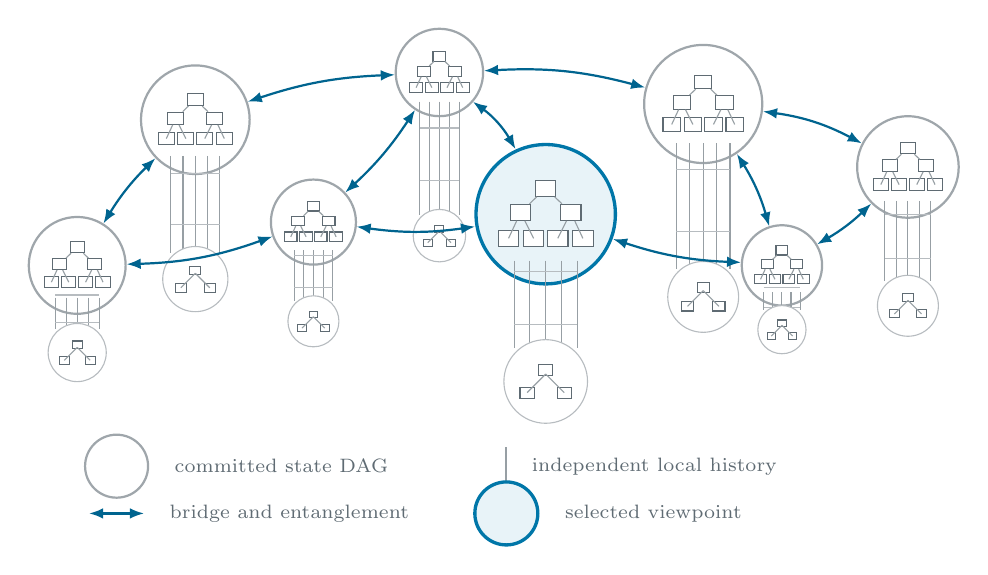
\begin{tikzpicture}[
  current/.style={circle, draw=swgray!60, thick, fill=white,
                  minimum size=15mm, inner sep=0pt},
  selected/.style={current, draw=swblue, very thick, fill=swlightblue},
  prior/.style={circle, draw=swgray!45, fill=white,
                minimum size=9mm, inner sep=0pt},
  dag node/.style={draw=swgray, fill=white, minimum width=2.2mm,
                   minimum height=1.7mm, inner sep=0pt},
  history strand/.style={draw=swgray!65, thin},
  bridge/.style={{Latex[length=1.8mm]}-{Latex[length=1.8mm]},
                 thick, draw=swblue!85!black},
  note/.style={font=\scriptsize, text=swgray, align=center},
]
  % #1 name, #2 x, #3 y, #4 history depth, #5 scale, #6 selected/current style
  \newcommand{\journalhistory}[6]{%
    \begin{scope}[shift={(#2,#3)}, scale=#5, transform shape]
      \node[#6] (#1) at (0,0) {};
      % Current state DAG.
      \node[dag node] (#1-r) at (0,0.28) {};
      \node[dag node] (#1-l) at (-0.27,0.02) {};
      \node[dag node] (#1-q) at (0.27,0.02) {};
      \node[dag node] at (-0.40,-0.26) {};
      \node[dag node] at (-0.13,-0.26) {};
      \node[dag node] at (0.13,-0.26) {};
      \node[dag node] at (0.40,-0.26) {};
      \draw[history strand] (#1-r)--(#1-l) (#1-r)--(#1-q);
      \draw[history strand] (#1-l)--(-0.40,-0.26) (#1-l)--(-0.13,-0.26);
      \draw[history strand] (#1-q)--(0.13,-0.26) (#1-q)--(0.40,-0.26);

      % Bundled structural continuity through local history.
      \foreach \x in {-0.34,-0.17,0,0.17,0.34} {
        \draw[history strand] (\x,-0.50) -- (\x,-#4+0.36);
      }
      \foreach \fraction in {0.34,0.66} {
        \draw[swgray!45, thin] (-0.34,{-#4*\fraction}) -- (0.34,{-#4*\fraction});
      }

      % Earlier retained state.
      \node[prior] (#1-old) at (0,-#4) {};
      \node[dag node, scale=0.7] at (0,{-#4+0.12}) {};
      \node[dag node, scale=0.7] at (-0.20,{-#4-0.12}) {};
      \node[dag node, scale=0.7] at (0.20,{-#4-0.12}) {};
      \draw[history strand] (0,{-#4+0.08}) -- (-0.20,{-#4-0.12});
      \draw[history strand] (0,{-#4+0.08}) -- (0.20,{-#4-0.12});
    \end{scope}%
  }

  % Eight independently advancing histories, intentionally heterogeneous.
  \journalhistory{jA}{-5.3}{-0.7}{1.35}{0.82}{current}
  \journalhistory{jB}{-3.8}{1.15}{2.20}{0.92}{current}
  \journalhistory{jC}{-2.3}{-0.15}{1.75}{0.72}{current}
  \journalhistory{jD}{-0.7}{1.75}{2.80}{0.74}{current}
  \journalhistory{jE}{0.65}{-0.05}{1.80}{1.18}{selected}
  \journalhistory{jF}{2.65}{1.35}{2.45}{1.00}{current}
  \journalhistory{jG}{3.65}{-0.70}{1.20}{0.68}{current}
  \journalhistory{jH}{5.25}{0.55}{2.05}{0.86}{current}

  % Sparse reciprocal bridge graph.  There is no enclosing global root.
  \draw[bridge] (jA) to[bend left=7] (jB);
  \draw[bridge] (jA) to[bend right=9] (jC);
  \draw[bridge] (jB) to[bend left=8] (jD);
  \draw[bridge] (jC) to[bend right=7] (jD);
  \draw[bridge] (jC) to[bend right=8] (jE);
  \draw[bridge] (jD) to[bend left=9] (jF);
  \draw[bridge] (jD) to[bend left=12] (jE);
  \draw[bridge] (jE) to[bend right=8] (jG);
  \draw[bridge] (jF) to[bend left=8] (jG);
  \draw[bridge] (jF) to[bend left=10] (jH);
  \draw[bridge] (jG) to[bend right=7] (jH);

  % Restrained two-row legend.
  \node[current, minimum size=8mm] (legend-state) at (-4.8,-3.25) {};
  \node[note, right=2mm of legend-state] {committed state DAG};
  \draw[history strand, thick] (0.15,-3.50) -- (0.15,-3.00);
  \node[note, right=2mm] at (0.15,-3.25) {independent local history};
  \draw[bridge] (-5.15,-3.85) -- (-4.45,-3.85);
  \node[note, right=2mm] at (-4.45,-3.85) {bridge and entanglement};
  \node[selected, minimum size=8mm] (legend-selected) at (0.15,-3.85) {};
  \node[note, right=2mm of legend-selected] {selected viewpoint};
\end{tikzpicture}
}
  \caption{The Synchronic Web}
  \label{fig:journal-relative-web}
\end{figure}

\section{Orientation and Scope}

A \emph{journal} is the software an entity runs together with all data persisted on it; it supplies that entity's root and operational viewpoint. A \emph{resource} is a path-addressed value or object whose low-level representation may be a leaf or a larger self-encoding structure. A \emph{bridge} relates independently maintained journals. People and applications should ordinarily read and write resources, invoke objects, follow links, and resolve history while specialized clients handle integrity evidence beneath those operations.

This paper is an architectural design and rationale, not an API guide or release-status report. Implemented mechanisms include the integrity substrate, partial structures, self-encoding objects, rooted paths, local histories, and core authorization machinery. Federation is partially implemented: the records layer contains reciprocal exchange, route segments and checkpoints, signed direct invocation, audience and watermark checks, route bounds, and key-index authorization, but it still requires end-to-end service testing and resolution of the gaps marked here. First-class links, general public application objects and queries, response binding, migration, and root recovery remain unsettled or unimplemented. The marker \WIP identifies claims that require implementation, renewed source inspection, or evaluation before this draft can become a specification.

Rooted paths, historical resolution, and bridge reachability already make the architecture Web-like in the limited sense of connecting independently administered resources from plural viewpoints. General hypermedia behavior depends on the unsettled first-class link semantics described in Chapter~5. The earlier Synchronic Web proposal shared the social purpose but used a different global synchronization architecture~\cite{dinh2023synchronic}; secure timelines and timeline entanglement are the direct lineage for the present bridge history~\cite{Maniatis2002timeline}.

\section{Trust and Adversaries}

The design assumes collision-resistant hashing, unforgeable digital signatures, canonical encoding for signed and hashed structures, and a verifier that begins from an explicitly accepted commitment. The trusted local base includes the client, evaluator, integrity primitives, operating-system execution boundary, runtime configuration, and key storage. Current root state persists interface private keys, so compromise of that protected state also compromises interface signing authority. Journal data storage may otherwise omit, replay, or substitute content without defeating integrity relative to an independently retained commitment, although it can destroy availability or roll an unwitnessed local anchor back. A malicious journal may sign false statements or present different valid branches; an intermediary may withhold, delay, or replay public proof material; and an unprotected network may observe or modify traffic. Integrity proofs detect inconsistency with an accepted commitment, not truthful semantics, complete disclosure, or availability.

Compromise timing matters. Previously witnessed signed heads and foreign incorporation receipts remain evidence of the branches that existed before compromise. Possession of a signing key can nevertheless authorize new heads and forks, and their detection still depends on comparison among witnesses. Loss of the initial non-rotating root key prevents ordinary authenticated continuation; compromise of that key threatens future continuity until a separately authenticated recovery protocol exists. Root-key recovery and rotation are unresolved parts of the design rather than assumptions hidden beneath indefinite identity.

\chapter{Integrity-Protected State}
\label{sec:integrity-state}
\label{sec:substrate}
\label{sec:partial-knowledge}

\section{Minimal Structural Model}

The native substrate is an integrity-verifiable binary data-structure DAG, following the general search-DAG model of authenticated structures~\cite{Martel2004general,Miller2014authenticated}. Leaves contain bytes, branches relate two children, and immutable substructure may be shared by many parents. At this layer there are no documents, users, histories, or bridges. Those concepts are constructed above a deliberately narrow vocabulary of roots, branches, leaves, stumps, and null.

The model distinguishes a \emph{logical digest} from a \emph{local handle}. The digest identifies recursively defined content or structure and is used for comparison and proof. The handle retrieves the representation available in one local store. Conflating the two would make storage placement part of logical identity and would prevent the same state from being represented under different persistence layouts.

\Cref{fig:dag-stump} shows the persisted forms. Roots map stable local names to node handles. Branches store child handles and the digest implied by their children. Leaves use a double hash so that their stored handle and logical content identity remain domain-separated from branch construction. A stump is unary persisted data that retains a logical digest when the corresponding structure is unavailable. Null is the all-zero word and denotes empty structure. These small forms are sufficient to construct all higher layers.

\begin{figure}[htbp]
  \centering
  \resizebox{\textwidth}{!}{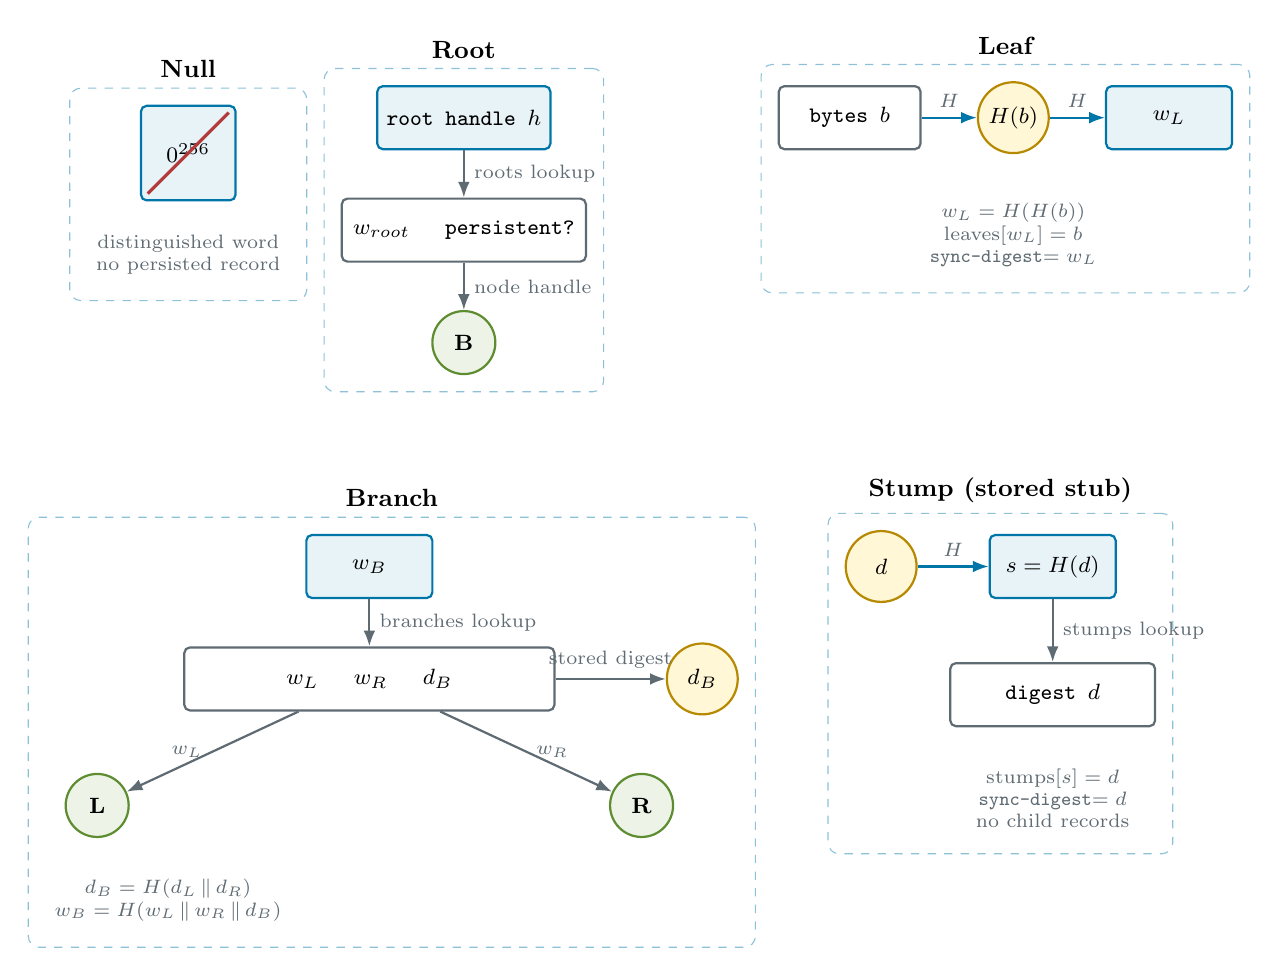
\begin{tikzpicture}[
  word/.style={draw=swblue, thick, rounded corners=2pt, fill=swlightblue,
               minimum width=16mm, minimum height=8mm, align=center, font=\footnotesize\ttfamily},
  record/.style={draw=swgray, thick, rounded corners=2pt, fill=white,
                 minimum width=18mm, minimum height=8mm, align=center, font=\footnotesize\ttfamily},
  dag node/.style={circle, draw=swgreen, thick, fill=swlightgreen,
                   minimum size=8mm, inner sep=1pt, font=\footnotesize\bfseries},
  digest/.style={circle, draw=swgold!85!black, thick, fill=swlightgold,
                 minimum size=9mm, inner sep=1pt, font=\footnotesize\ttfamily},
  lookup/.style={-{Latex[length=2mm]}, thick, draw=swgray},
  hash/.style={-{Latex[length=2mm]}, thick, draw=swblue},
  panel/.style={draw=swblue!45, rounded corners=4pt, dashed, inner sep=6pt},
  note/.style={font=\scriptsize, text=swgray, align=center},
]
  % Null --------------------------------------------------------------------
  \node[word, minimum size=12mm] (nullword) at (1.7,0) {$0^{256}$};
  \draw[swred, very thick] ($(nullword.south west)+(1mm,1mm)$) -- ($(nullword.north east)+(-1mm,-1mm)$);
  \node[note, below=3mm of nullword] (nullnote) {distinguished word\\no persisted record};
  \node[panel, fit=(nullword)(nullnote), label={[font=\small\bfseries]above:Null}] (nullpanel) {};

  % Root --------------------------------------------------------------------
  \node[word] (roothandle) at (5.2,0.45) {root handle $h$};
  \node[record, below=6mm of roothandle, minimum width=31mm] (rootrecord) {$w_{root}$ \quad persistent?};
  \node[dag node, below=6mm of rootrecord] (rootbranch) {B};
  \draw[lookup] (roothandle) -- node[right,note] {roots lookup} (rootrecord);
  \draw[lookup] (rootrecord) -- node[right,note] {node handle} (rootbranch);
  \node[panel, fit=(roothandle)(rootrecord)(rootbranch),
        label={[font=\small\bfseries]above:Root}] (rootpanel) {};

  % Leaf --------------------------------------------------------------------
  \node[record] (leafbytes) at (10.1,0.45) {bytes $b$};
  \node[digest, right=7mm of leafbytes] (leafhashone) {$H(b)$};
  \node[word, right=7mm of leafhashone] (leafhandle) {$w_L$};
  \draw[hash] (leafbytes) -- node[above,note] {$H$} (leafhashone);
  \draw[hash] (leafhashone) -- node[above,note] {$H$} (leafhandle);
  \node[note, below=5mm of leafhashone] (leafnote) {$w_L=H(H(b))$\\leaves$[w_L]=b$\\\texttt{sync-digest}$=w_L$};
  \node[panel, fit=(leafbytes)(leafhashone)(leafhandle)(leafnote),
        label={[font=\small\bfseries]above:Leaf}] (leafpanel) {};

  % Branch ------------------------------------------------------------------
  \node[word] (branchhandle) at (4.0,-5.25) {$w_B$};
  \node[record, below=6mm of branchhandle, minimum width=47mm] (branchrecord)
    {$w_L$ \quad $w_R$ \quad $d_B$};
  \node[dag node, below left=9mm and 8mm of branchrecord] (leftchild) {L};
  \node[dag node, below right=9mm and 8mm of branchrecord] (rightchild) {R};
  \node[digest, right=14mm of branchrecord] (branchdigest) {$d_B$};
  \draw[lookup] (branchhandle) -- node[right,note] {branches lookup} (branchrecord);
  \draw[lookup] ($(branchrecord.south)+(-9mm,0)$) -- node[left,note] {$w_L$} (leftchild);
  \draw[lookup] ($(branchrecord.south)+(9mm,0)$) -- node[right,note] {$w_R$} (rightchild);
  \draw[lookup] (branchrecord) -- node[above,note] {stored digest} (branchdigest);
  \node[note, below=4mm of leftchild, xshift=9mm] (branchnote)
    {$d_B=H(d_L\,\|\,d_R)$\\$w_B=H(w_L\,\|\,w_R\,\|\,d_B)$};
  \node[panel, fit=(branchhandle)(branchrecord)(leftchild)(rightchild)(branchdigest)(branchnote),
        label={[font=\small\bfseries]above:Branch}] (branchpanel) {};

  % Stump -------------------------------------------------------------------
  \node[digest] (stumpdigest) at (10.5,-5.25) {$d$};
  \node[word, right=9mm of stumpdigest] (stumphandle) {$s=H(d)$};
  \node[record, below=8mm of stumphandle, minimum width=26mm] (stumprecord) {digest $d$};
  \draw[hash] (stumpdigest) -- node[above,note] {$H$} (stumphandle);
  \draw[lookup] (stumphandle) -- node[right,note] {stumps lookup} (stumprecord);
  \node[note, below=4mm of stumprecord] (stumpnote)
    {stumps$[s]=d$\\\texttt{sync-digest}$=d$\\no child records};
  \node[panel, fit=(stumpdigest)(stumphandle)(stumprecord)(stumpnote),
        label={[font=\small\bfseries]above:Stump (stored stub)}] (stumppanel) {};
\end{tikzpicture}
}
  \caption{Persisted DAG Node Forms}
  \label{fig:dag-stump}
\end{figure}

\section{Commitment and Reachability}

A digest commits to the complete logical structure recursively defined beneath it. Replacing a leaf changes every dependent ancestor digest, so modification produces a new state rather than altering the identity of the old one. A durable root is consequently a mutable local reference to immutable identified structure: advancing a root selects a successor state while leaving its predecessor independently identifiable.

Verification must still begin from a commitment that the verifier has accepted through authentication, prior observation, or local policy. The structure can prove that available material is consistent with that commitment. It cannot prove who created the commitment, whether the signer is meaningful to the verifier, or whether the state is true. Those are separate identity and policy questions.

Logical reachability and material possession are also distinct. Data may be fully available, represented only by stubs, persisted locally but no longer reachable from a root, or absent from the local store. Garbage collection can change local possession without changing a commitment retained by another observer. No integrity mechanism can reconstruct bytes that no one retains; availability ultimately depends on replication and operational preservation.

\section{Partial Knowledge}

Different observers need not possess the same portions of an identified state. The architecture distinguishes known content, semantic absence, unresolved content without a commitment, and identified structure whose contents are unavailable or intentionally undisclosed. False, empty, missing, unknown, and pruned values therefore cannot be treated as interchangeable sentinels.

A stub retains the logical digest of missing structure, while a stump is the corresponding persisted low-level representation. The stub states exactly what structure belongs at a position, but says nothing about why it is missing or whether it can be recovered. Traversal stops at that point until the observer obtains replacement evidence with the same digest. Null, by contrast, denotes actual empty structure rather than unavailable content.

Making stubs first-class permits integrity to survive selective disclosure and local pruning. An observer can know where unavailable material belongs in a larger state and can later verify a compatible replacement without having learned the material in the meantime. Partial knowledge is thus a property of possession, not a different logical state.

\section{Slice, Prune, and Merge}

Slicing retains evidence along selected paths and replaces unrelated material with digest-preserving stubs. The result has the same root digest as the complete source and is therefore a partial representation of that state, not a newly computed summary. Compact Merkle multiproofs likewise remove redundant evidence~\cite{Ramabaja2020compact}; object-aware slicing additionally crosses documented semantic boundaries rather than traversing only physical branch positions.

\begin{algorithm}[htbp]
\caption{Deep Slice Along Object Path}
\label{alg:deep-slice}
\begin{algorithmic}[1]
\Require Object node $x$ and nonempty path $p$
\Ensure The selected path remains available and the logical digest is unchanged
\Function{DeepSlice}{$x,p$}
  \State $o \gets \Call{EvaluateObject}{x}$
  \State $k \gets \Call{First}{p}$
  \If{$|p| = 1$}
    \State $o.\Call{Slice}{k}$
    \State \Return $\Call{Node}{o}$
  \EndIf
  \State $c \gets o.\Call{Get}{k}$
  \State $d \gets \Call{Digest}{c}$
  \State $q \gets \Call{Rest}{p}$
  \State $c' \gets \Call{DeepSlice}{c,q}$
  \If{$\Call{Digest}{c'} \ne d$}
    \State \Call{Fail}{``slice changed child digest''}
  \EndIf
  \State $o.\Call{Set}{k,c'}$
  \State $o.\Call{Slice}{k}$ \Comment{discard siblings not needed for $k$}
  \State \Return $\Call{Node}{o}$
\EndFunction
\end{algorithmic}
\end{algorithm}


Pruning performs the complementary local operation. It intentionally replaces available material with a stub of the same digest, reducing possession while preserving the old logical identity. This differs from deletion, which changes the state. Controlled deletion in tamper-evident logs provides a related retention precedent~\cite{Crosby2009efficient}; structural pruning applies the distinction throughout a composable DAG.

\begin{algorithm}[htbp]
\caption{Deep Prune Along Object Path}
\label{alg:deep-prune}
\begin{algorithmic}[1]
\Require Object node $x$ and nonempty path $p$
\Ensure Evidence at the selected path is removed without changing the logical digest
\Function{DeepPrune}{$x,p$}
  \State $o \gets \Call{EvaluateObject}{x}$
  \State $k \gets \Call{First}{p}$
  \If{$|p| = 1$}
    \State $o.\Call{Prune}{k}$
    \State \Return $\Call{Node}{o}$
  \EndIf
  \State $c \gets o.\Call{Get}{k}$
  \If{$c$ is not an available pair node}
    \State \Return $\Call{Node}{o}$
  \EndIf
  \State $d \gets \Call{Digest}{c}$
  \State $q \gets \Call{Rest}{p}$
  \State $c' \gets \Call{DeepPrune}{c,q}$
  \If{$\Call{Digest}{c'} \ne d$}
    \State \Call{Fail}{``prune changed child digest''}
  \EndIf
  \If{$c'$ is a stub}
    \State $o.\Call{Prune}{k}$
  \Else
    \State $o.\Call{Set}{k,c'}$
  \EndIf
  \State \Return $\Call{Node}{o}$
\EndFunction
\end{algorithmic}
\end{algorithm}


Merge combines complementary partial representations only when their commitments agree. Available material may replace a stub with the same digest, and two available branches may be merged recursively. A disagreement in digest fails immediately rather than selecting a preferred source, because the inputs then describe different logical states. Merge can therefore increase possession without changing state identity; it is not an application-level conflict-resolution policy.

\begin{algorithm}[htbp]
\caption{Merge Compatible Partial Structures}
\label{alg:merge-partial}
\begin{algorithmic}[1]
\Require Partial structures $a$ and $b$
\Ensure The result contains the union of available evidence and retains the common digest
\Function{MergePartial}{$a,b$}
  \If{$\Call{Digest}{a} \ne \Call{Digest}{b}$}
    \State \Call{Fail}{``cannot merge different digests''}
  \EndIf
  \If{$a$ is null}
    \State \Return $a$
  \ElsIf{$a$ is a byte-vector leaf}
    \State \Return $a$
  \ElsIf{$a$ is a stub}
    \State \Return $b$
  \ElsIf{$b$ is a stub}
    \State \Return $a$
  \Else
    \State $a_L \gets \Call{Left}{a}$; $b_L \gets \Call{Left}{b}$
    \State $a_R \gets \Call{Right}{a}$; $b_R \gets \Call{Right}{b}$
    \State $l \gets \Call{MergePartial}{a_L,b_L}$
    \State $r \gets \Call{MergePartial}{a_R,b_R}$
    \State \Return $\Call{Pair}{l,r}$
  \EndIf
\EndFunction
\end{algorithmic}
\end{algorithm}


\section{Transport and Incremental Evidence}

Serialization records node kinds, byte contents, and retained digests so that deserialization reconstructs the same logical root before any merge or evaluation occurs. The transport framing and compression are replaceable as long as this round trip remains exact. A query-shaped traversal may therefore send only the structure touched by a read, while a later request supplies another compatible slice from the same committed state.

This incremental model supports ordinary resource access. A client can accept a root, obtain proof for one resource, verify and retain the partial representation, and later merge additional evidence. A valid slice or successful merge still proves only consistency. It does not establish that the root is authoritative, that omitted content is harmless, or that missing material will remain obtainable. Specialized clients should hide proof construction and merging beneath normal reads while preserving these distinctions in their error reporting.

Resource limits remain necessary at the transport boundary. Structurally valid evidence can be adversarially deep, broad, or expensive to decode. Verification therefore requires bounds on encoded size, node count, recursion, allocation, and traversal work in addition to cryptographic checks.

\section{Why the Substrate Is Small}

A narrow trusted base fixes construction, hashing, persistence, and controlled evaluation while leaving maps, histories, objects, and policy inspectable and replaceable above it. Rich native record types would improve immediate convenience, but each would make semantic evolution a privileged runtime change. At the other extreme, a content-addressed blob store can identify complete values but cannot independently slice and merge their internal structure.

Conventional serialization similarly preserves bytes without making arbitrary partial representations verifiable against one identity. Operations therefore belong in the native substrate only when higher layers cannot express them safely or efficiently. This minimality is a boundary discipline rather than an aesthetic end: the foundation should be small enough to audit while still supporting the structural proofs and controlled evaluation on which every higher abstraction depends.

\chapter{History and Entanglement}
\label{sec:history-entanglement}
\label{sec:historical-structure}
\label{sec:bridges}

\section{From Mutation to History}

A journal separates proposed state from committed history. Applications may accumulate staged mutations, inspect their effects, and abandon or replace them before a step selects the next historically resolvable state. The step is therefore a semantic boundary, not merely a storage flush. It records transition context, advances the history, signs the resulting head, and applies retention policy as one controlled operation.

Environmental values do not enter durable behavior implicitly. Time, remote responses, randomness, and operator choices are prepared as explicit inputs before the step. If those inputs and the proposed application state do not produce a meaningful change, the mechanism need not append an empty historical entry. When it does append, altering prior material later either creates another branch or breaks verification; it cannot retroactively change the state formerly identified. Linked cryptographic timestamping established this distinction between detectable rewriting and physically immutable media~\cite{Haber1991timestamp}.

\section{Committed Steps}

Committed states are index-addressable within a persistent chain, following persistent integrity-verifiable dictionaries and tamper-evident histories~\cite{Anagnostopoulos2001persistent,Crosby2009efficient}. Each chain entry points to a tree that contains application state, declared transition information, retained foreign heads, and signing material. All of these components ultimately reduce to the persisted forms described in \cref{fig:dag-stump}.

Transition records describe the journal's declared operation and explicit inputs. They provide a durable place for provenance without imposing one universal application vocabulary. A supply-chain event, document edit, and agent observation may all require different semantic descriptions even though they share one historical structure. Likewise, a head signature authenticates control of a signing key over that commitment but does not by itself make the key a meaningful principal. Identity depends on how the key is resolved through history and interpreted by local policy.

\Cref{fig:step-anatomy} separates the logical chain from the contents of one step. The corresponding procedure in Algorithm~\ref{alg:commit-step} compares staged and prior state, records explicit transition context, incorporates eligible retained material, signs the successor, and advances the durable root only after successful construction.

\begin{figure}[htbp]
  \centering
  \resizebox{0.96\textwidth}{!}{% Logical contents of one committed step.  Application paths are nested beneath
% *state*; cryptographic/public-descriptor fields are intentionally simplified.
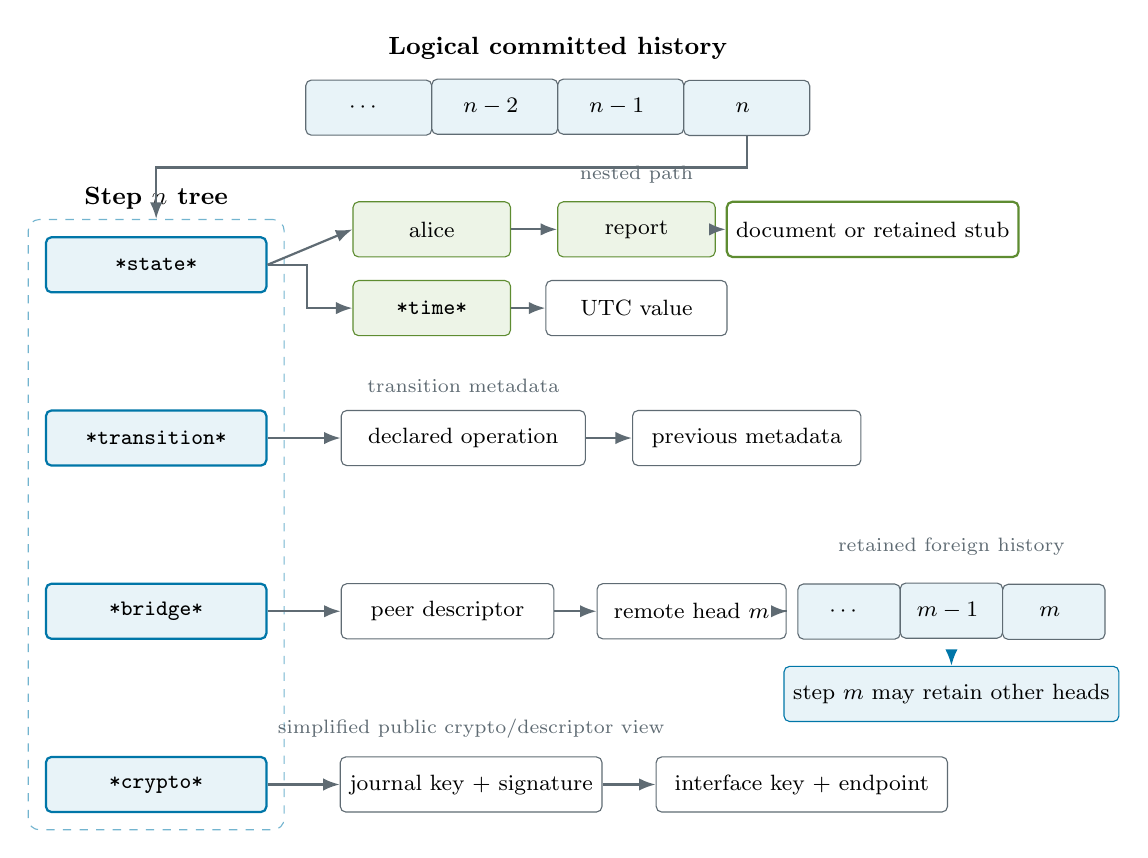
\begin{tikzpicture}[
  box/.style={draw=swgray, rounded corners=2pt, fill=white,
              minimum height=7mm, align=center, font=\footnotesize},
  ns/.style={box, draw=swblue, thick, fill=swlightblue, minimum width=28mm,
             font=\footnotesize\ttfamily},
  data/.style={box, draw=swgreen, fill=swlightgreen, minimum width=20mm},
  history/.style={box, fill=swlightblue, minimum width=16mm},
  group/.style={draw=swblue!55, rounded corners=4pt, dashed, inner sep=6pt},
  arrow/.style={-{Latex[length=2.1mm]}, thick, draw=swgray},
  recur/.style={arrow, dashed, draw=swblue},
  note/.style={font=\scriptsize, text=swgray, align=center},
]
  % Local history and selected step.
  \matrix (chain) [matrix of nodes, nodes={history}, column sep=-\pgflinewidth,
                   label={[font=\small\bfseries]above:Logical committed history}] at (0,0) {
    $\cdots$ & $n-2$ & $n-1$ & $n$ \\
  };

  \node[ns] (state-ns) at (-5.1,-2.0) {\texttt{*state*}};
  \node[ns] (trans-ns) at (-5.1,-4.2) {\texttt{*transition*}};
  \node[ns] (bridge-ns) at (-5.1,-6.4) {\texttt{*bridge*}};
  \node[ns] (crypto-ns) at (-5.1,-8.6) {\texttt{*crypto*}};
  \node[group, fit=(state-ns)(trans-ns)(bridge-ns)(crypto-ns),
        label={[font=\small\bfseries]above:Step $n$ tree}] (step) {};
  \draw[arrow] (chain-1-4.south) -- ++(0,-4mm) -| (step.north);

  % Correct nested application path: (*state* alice report).
  \node[data] (alice) at (-1.6,-1.55) {alice};
  \node[data] (report) at (1.0,-1.55) {report};
  \node[box, draw=swgreen, thick, minimum width=32mm] (document) at (4.0,-1.55)
    {document or retained stub};
  \node[data, font=\footnotesize\ttfamily] (time-key) at (-1.6,-2.55) {\texttt{*time*}};
  \node[box, minimum width=23mm] (time-value) at (1.0,-2.55) {UTC value};
  \draw[arrow] (state-ns.east) -- (alice.west);
  \draw[arrow] (alice.east) -- (report.west);
  \draw[arrow] (report.east) -- (document.west);
  \draw[arrow] (state-ns.east) -- ++(5mm,0) |- (time-key.west);
  \draw[arrow] (time-key.east) -- (time-value.west);
  \node[note, above=1mm of report] {nested path};

  % Declared transition metadata, not an exhaustive provenance log.
  \node[box, minimum width=31mm] (declared) at (-1.2,-4.2) {declared operation};
  \node[box, minimum width=29mm] (previous) at (2.4,-4.2) {previous metadata};
  \draw[arrow] (trans-ns.east) -- (declared.west);
  \draw[arrow] (declared.east) -- (previous.west);
  \node[note, above=1mm of declared] {transition metadata};

  % Retained foreign history can recursively contain other heads.
  \node[box, minimum width=27mm] (peer) at (-1.4,-6.4) {peer descriptor};
  \node[box, minimum width=24mm] (remote-head) at (1.7,-6.4) {remote head $m$};
  \matrix (remote) [matrix of nodes, nodes={history, minimum width=13mm},
                    column sep=-\pgflinewidth] at (5.0,-6.4) {
    $\cdots$ & $m-1$ & $m$ \\
  };
  \draw[arrow] (bridge-ns.east) -- (peer.west);
  \draw[arrow] (peer.east) -- (remote-head.west);
  \draw[arrow] (remote-head.east) -- (remote.west);
  \node[note, above=1mm of remote] {retained foreign history};
  \node[box, draw=swblue, fill=swlightblue, minimum width=34mm] (nested) at (5.0,-7.45)
    {step $m$ may retain other heads};
  \draw[recur] (remote.south) -- (nested.north);

  % Deliberately simplified public cryptographic/descriptor view.
  \node[box, minimum width=33mm] (journal-crypto) at (-1.1,-8.6)
    {journal key + signature};
  \node[box, minimum width=37mm] (interface-crypto) at (3.1,-8.6)
    {interface key + endpoint};
  \draw[arrow] (crypto-ns.east) -- (journal-crypto.west);
  \draw[arrow] (journal-crypto.east) -- (interface-crypto.west);
  \node[note, above=1mm of journal-crypto] {simplified public crypto/descriptor view};
\end{tikzpicture}
}
  \caption{Committed Step Anatomy}
  \label{fig:step-anatomy}
\end{figure}

\begin{algorithm}[htbp]
\caption{Commit Journal Step}
\label{alg:commit-step}
\small
\begin{algorithmic}[1]
\Require Ledger $L$, Unix time $t$, signing public key $p_k$, signing secret key $s_k$
\Ensure Either no step is needed or a signed step is appended and retention is updated
\Function{CommitStep}{$L,t,p_k,s_k$}
  \Statex \Comment{Comparable state omits transition and cryptographic metadata.}
  \State $(S,P,T) \gets \Call{EvaluateLedgerFields}{L}$
  \State $d_{cur} \gets \Call{ComparableStateDigest}{S}$
  \If{$\Call{Size}{P}=0$}
    \State $d_{prev} \gets \Call{Digest}{\mathit{null}}$
  \Else
    \State $h \gets \Call{Get}{P,-1}$
    \State $d_{prev} \gets \Call{ComparableStateDigest}{h}$
  \EndIf
  \If{$d_{cur}=d_{prev}$}
    \State \Return $\Call{Size}{P}$
  \EndIf
  \State $u \gets \Call{UTC}{t}$
  \State $S.\Call{RecordTransition}{[\texttt{*state*},\texttt{*time*}],u}$
  \State $P.\Call{Push}{\operatorname{Node}(S)}$
  \State $S.\Call{Delete}{\texttt{*transition*}}$
  \State $P.\Call{SignHead}{p_k,s_k}$
  \State $T.\Call{Push}{P[-1]}$
  \State $q_t \gets \Call{DeepSlice}{\operatorname{Node}(T),[-1,\texttt{*state*/*time*}]}$
  \If{$L.\mathit{window}$ is set and $\Call{Size}{T}>L.\mathit{window}$}
    \State $T.\Call{Prune}{-(L.\mathit{window}+1)}$
  \EndIf
  \State $q_p \gets \Call{DeepPrune}{\operatorname{Node}(P),[-1,\texttt{*state*}]}$
  \State $L.\mathit{stage} \gets \operatorname{Node}(S)$
  \State $L.\mathit{permanent} \gets \Call{MergePartial}{q_t,q_p}$
  \State $L.\mathit{temporary} \gets \operatorname{Node}(T)$
  \State \Return $\Call{Size}{P}$
\EndFunction
\end{algorithmic}
\end{algorithm}


\section{Retention and Pinning}

Structural commitment and material retention are independent decisions. A journal may keep recent heads in complete form while permanent history retains only chain continuity, signatures, selected proofs, and explicitly pinned resources. The discarded material remains part of the logical state even when the local journal now holds only its digest.

Pinning merges a compatible slice into the evidence retained for history. Unpinning releases that local retention obligation; it does not delete the historical commitment or affect copies held by other journals. Retention policy therefore governs local availability rather than global survival. Replication, media renewal, and institutional preservation remain separate operational commitments.

Historical resolution follows directly from this model. The same resource coordinate can be evaluated against different committed heads, and each result can carry only the evidence needed for that particular path. A client may know that a resource existed at one index even when most unrelated state from that index has been pruned.

\section{Reciprocal Bridges}

\WIP A bridge is a reciprocal, cryptographically verified relationship in which each journal retains a verified head and public descriptor for the other. Reciprocity makes history and public identity reachable in both directions, but it grants no authority over application data. The relationship is a public control-plane connection, not a replication permission.

The journal that creates a bridge becomes its ongoing synchronization initiator unless administrators explicitly renegotiate the role. The initial design has no alternating or dual-initiator mode. This asymmetry in scheduling does not imply authority: one exchange still carries both heads. It allows private or intermittently reachable journals to maintain reciprocal relationships using outbound connectivity alone.

Establishment exchanges root-signed heads and descriptors in both directions. Those signed objects authenticate bridge creation independently of the later federated-invocation envelope. An acceptor may admit a valid request automatically when the creator retains initiation responsibility, or a locked-down deployment may require prior approval of the creator's stable root key. Invalid or unmatched requests are rejected without creating durable pending state. Because even an accepted public relationship consumes storage and verification work, automatic admission still requires rate and resource bounds.

\section{Reciprocal Synchronization}

\WIP One replay-safe request and response synchronize both current heads, as shown in \cref{fig:bridge-reciprocal}. The initiator sends its root-signed head and continuity context. The acceptor verifies that evidence, stages the head, and returns its own root-signed head. The initiator then performs the same verification and staging locally. Every path must check the stable root signature, predecessor continuity, expected peer identity, disclosure scope, freshness conditions, and resource limits.

Repeating an already accepted exchange is idempotent. Acceptance itself is not yet historical incorporation: each journal commits the staged foreign head only in a later local step. Neither party can force the other's step cadence, which avoids turning remote traffic into control over local serialization or an inexpensive denial-of-service mechanism. \WIP The exact acknowledgement, incorporation-proof retrieval, and failure-recovery protocol remains unsettled.

\begin{figure}[htbp]
  \centering
  \resizebox{\textwidth}{!}{\begin{sequencediagram}
  \tikzset{every node/.append style={font=\small}}
  \tikzstyle{inststyle}+=[draw=swblue,fill=swlightblue,drop shadow={opacity=0}]

  \newthread{schedule}{Initiator scheduler}
  \newinst[1.25]{ijournal}{Initiator journal}
  \newinst[1.55]{ainterface}{Acceptor interface}
  \newinst[1.25]{ajournal}{Acceptor journal}

  \begin{call}[2]{schedule}{prepare root-signed head $A$}{ijournal}{head $A$; continuity context}
  \end{call}

  \begin{call}[3]{schedule}{reciprocal head exchange}{ainterface}{root-signed head $B$; acceptance}
    \begin{call}[2]{ainterface}{verify root signature and stage $A$}{ajournal}{root-signed head $B$}
    \end{call}
  \end{call}

  \begin{call}[2]{schedule}{verify root signature and stage $B$}{ijournal}{accepted context}
  \end{call}

\end{sequencediagram}
}
  \caption{Bidirectional Head Exchange}
  \label{fig:bridge-reciprocal}
\end{figure}

\section{Cross-Timeline Ordering}

Suppose journal B accepts a signed head from journal A and later includes it in B's own committed state. A's past has then become an input to B's future: the included A head must predate B's incorporating head. B's later head together with an inclusion proof is an incorporation receipt. The earlier staging acknowledgement is not, because it proves no committed cross-timeline ordering.

Repeated incorporation can weave independent histories together without producing one consensus sequence. This is the central result of timeline entanglement: temporal mappings and receipts can remain verifiable after an originating service disappears or refuses further cooperation~\cite{Maniatis2002timeline}. The mapping is necessarily coarse. Because synchronization and commit cadences differ, an event in A generally maps to an interval in B rather than to one exact shared instant.

\WIP The reciprocal protocol must represent accepted, incorporated, and acknowledged heads distinctly. Collapsing these states would overstate the meaning of an exchange and obscure recovery after partial failure. \Cref{fig:entangled-state} contrasts the two relationships involved: deterministic computation transforms explicit local state and arguments, while entanglement persists a foreign commitment within another journal's later state.

\section{Recursive History and Forks}

A retained foreign head may itself include other heads, allowing historical reachability to compose recursively while every journal preserves its own ordering and viewpoint. This transitivity is structural, not political. A journal may verify that a distant history is connected through intermediate commitments without trusting those intermediaries, endorsing the distant journal, or granting it application authority.

A signature and continuity proof establish one valid branch, not uniqueness. A dishonest journal can present distinct signed branches to isolated peers. Cross-inclusions can preserve contradictory evidence once the branches meet, but detection requires independent witnesses or transparency overlays to compare signed views~\cite{Maniatis2002timeline,Chase2016transparency}. Fork evidence is therefore different from fork prevention.

Timeline entanglement supplies the established cross-history mechanism. The larger Synchronic Web setting adds executable, partially retained, path-addressable state around it~\cite{dinh2023composable}. Histories can consequently carry ordinary resources and durable interpretation, not only timeline authenticators.

\begin{figure}[htbp]
  \centering
  \resizebox{0.94\textwidth}{!}{% Three journal-relative views.  The highlighted heads from journals A and B
% reappear as retained foreign commitments inside a later state of journal C.
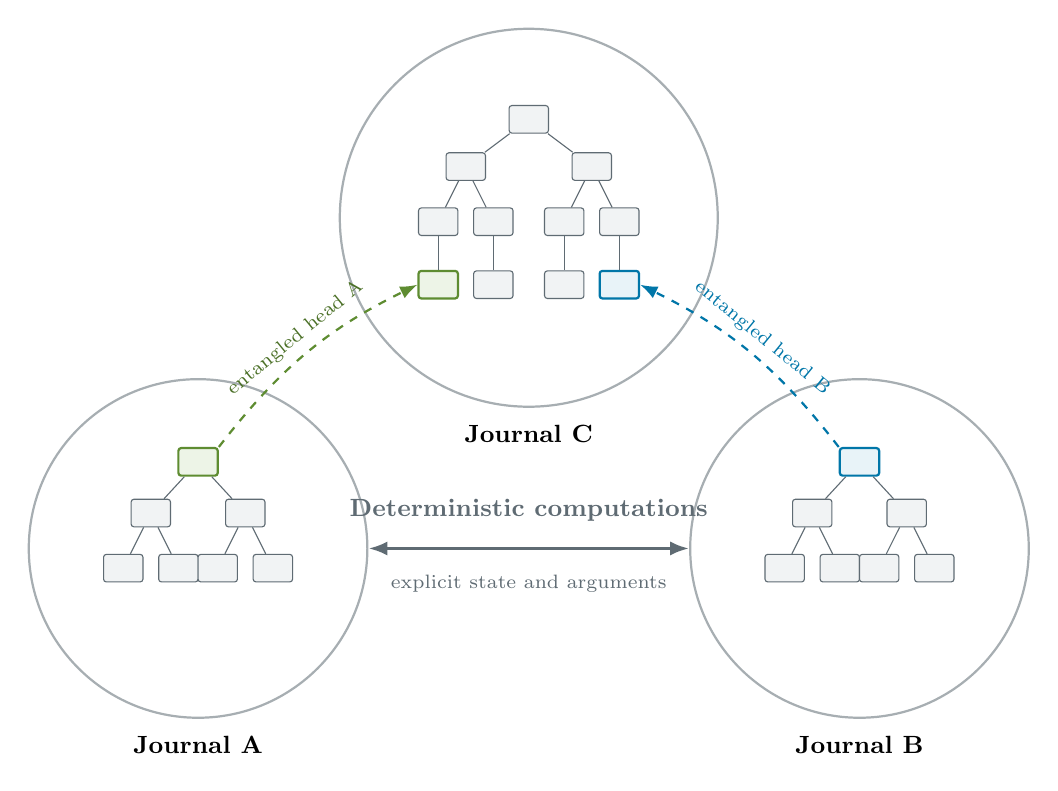
\begin{tikzpicture}[
  view/.style={circle, draw=swgray!55, thick, fill=white,
               minimum size=43mm, inner sep=2mm},
  inode/.style={draw=swgray, rounded corners=1pt, fill=swlightgray,
                minimum width=5mm, minimum height=3.5mm, inner sep=0pt},
  branch/.style={draw=swgray, thin},
  entangle a/.style={-{Latex[length=2.2mm]}, thick, dashed, draw=swgreen},
  entangle b/.style={-{Latex[length=2.2mm]}, thick, dashed, draw=swblue},
  compute/.style={{Latex[length=2.4mm]}-{Latex[length=2.4mm]}, very thick, draw=swgray},
  note/.style={font=\scriptsize, align=center, text=swgray},
]
  % Journal A ---------------------------------------------------------------
  \node[view] (aview) at (-4.2,-2.0) {};
  \node[inode, draw=swgreen, thick, fill=swlightgreen] (aroot) at (-4.2,-0.9) {};
  \node[inode] (a1) at (-4.8,-1.55) {};
  \node[inode] (a2) at (-3.6,-1.55) {};
  \node[inode] (a3) at (-5.15,-2.25) {};
  \node[inode] (a4) at (-4.45,-2.25) {};
  \node[inode] (a5) at (-3.95,-2.25) {};
  \node[inode] (a6) at (-3.25,-2.25) {};
  \draw[branch] (aroot)--(a1) (aroot)--(a2);
  \draw[branch] (a1)--(a3) (a1)--(a4) (a2)--(a5) (a2)--(a6);
  \node[font=\small\bfseries, below=1mm of aview.south] {Journal A};

  % Journal B ---------------------------------------------------------------
  \node[view] (bview) at (4.2,-2.0) {};
  \node[inode, draw=swblue, thick, fill=swlightblue] (broot) at (4.2,-0.9) {};
  \node[inode] (b1) at (3.6,-1.55) {};
  \node[inode] (b2) at (4.8,-1.55) {};
  \node[inode] (b3) at (3.25,-2.25) {};
  \node[inode] (b4) at (3.95,-2.25) {};
  \node[inode] (b5) at (4.45,-2.25) {};
  \node[inode] (b6) at (5.15,-2.25) {};
  \draw[branch] (broot)--(b1) (broot)--(b2);
  \draw[branch] (b1)--(b3) (b1)--(b4) (b2)--(b5) (b2)--(b6);
  \node[font=\small\bfseries, below=1mm of bview.south] {Journal B};

  % Journal C, containing retained heads from A and B -----------------------
  \node[view, minimum size=48mm] (cview) at (0,2.2) {};
  \node[inode] (croot) at (0,3.45) {};
  \node[inode] (c1) at (-0.8,2.85) {};
  \node[inode] (c2) at (0.8,2.85) {};
  \node[inode] (c3) at (-1.15,2.15) {};
  \node[inode] (c4) at (-0.45,2.15) {};
  \node[inode] (c5) at (0.45,2.15) {};
  \node[inode] (c6) at (1.15,2.15) {};
  \node[inode, draw=swgreen, thick, fill=swlightgreen] (ca) at (-1.15,1.35) {};
  \node[inode] (c7) at (-0.45,1.35) {};
  \node[inode] (c8) at (0.45,1.35) {};
  \node[inode, draw=swblue, thick, fill=swlightblue] (cb) at (1.15,1.35) {};
  \draw[branch] (croot)--(c1) (croot)--(c2);
  \draw[branch] (c1)--(c3) (c1)--(c4) (c2)--(c5) (c2)--(c6);
  \draw[branch] (c3)--(ca) (c4)--(c7) (c5)--(c8) (c6)--(cb);
  \node[font=\small\bfseries, below=1mm of cview.south] {Journal C};

  % Cross-view relations ----------------------------------------------------
  \draw[entangle a] (aroot.north east) to[bend left=13]
    node[sloped, above, note, text=swgreen!80!black] {entangled head A} (ca.west);
  \draw[entangle b] (broot.north west) to[bend right=13]
    node[sloped, above, note, text=swblue] {entangled head B} (cb.east);
  \draw[compute] (aview.east) -- node[above=2mm, font=\small\bfseries, text=swgray]
    {Deterministic computations}
    node[below=2mm, note] {explicit state and arguments} (bview.west);
\end{tikzpicture}
}
  \caption{Computation and Entangled State}
  \label{fig:entangled-state}
\end{figure}

\chapter{Self-Encoding Structure}
\label{sec:self-encoding}
\label{sec:objects}
\label{sec:sandbox}
\label{sec:semantic-bootstrapping}

\section{Code at Web Scale}

A durable network must survive software change as well as storage failure. Data written today may be read by another organization years later, after schemas, libraries, runtimes, and deployment practices have moved on; preserving bytes answers only the first half of the archival question, because the reader also needs a durable account of how those bytes were structured and what operations gave them meaning. The Web already offers several approaches: JavaScript carries behavior to a widely available runtime, Protocol Buffers and similar schema-driven encodings define stable wire forms and evolution rules whose schemas supply interpretation beyond each payload, package managers and containers capture dependencies, and reproducible-build and software-transparency systems make artifacts traceable to declared sources and environments~\cite{Nikitin2017chainiac}. Each binds a different portion of the path from stored bits to behavior. At Web scale, change management crosses administrative boundaries: a recipient may accept data while declining the producer's newest software, or retain an old object long after its originating service has migrated. Reproducibility also demands explicit treatment of time, randomness, network responses, and operator choices. Self-encoding structure answers these pressures by placing a changeable definition inside the same commitment as the state it interprets, creating a historical pair that can travel, be sliced, and be cited together. The runtime becomes a smaller shared foundation, application semantics become ordinary versioned material, and transitions can expose the environmental inputs on which their results depend.

\section{Lisp as Durable Structure}

Lisp gives code and data one inspectable representation: a method definition, query, path, transition, or configuration is an expression that can be hashed, stored, transmitted, and evaluated. Homoiconicity turns semantic bootstrapping into structural composition because the network can preserve the form describing an operation with the same substrate that preserves its inputs. The implemented runtime uses s7 Scheme inside the journal; native primitives provide construction, hashing, persistence, slicing, network preparation, and controlled evaluation, while Scheme builds maps, chains, ledgers, authorization, and object protocols above them. This follows the tier-unifying intuition of single-language Web systems~\cite{Cooper2007links}, preserving explicit boundaries while reducing translations between durable state and the logic that uses it. The bootstrap terminates in native storage and evaluator semantics, which define how expressions are read, nodes are hashed, primitives are exposed, and resources are bounded. Keeping this foundation small makes it practical to inspect and reproduce while every higher layer can evolve as identified structure in journal history. A shared language still permits heterogeneous protocols: objects may implement different methods and evolve under different authorities while remaining transportable through the same node and evaluator model, with documented public behavior providing compatibility across class systems. \WIP Per-object capability assignment would extend the current shared reduced evaluation environment.

\section{Self-Encoding Objects}

A standard object is a node with executable definition on the left and durable state on the right; its digest commits to both components and to their association. Evaluating that node with \texttt{sync-eval} produces a transient callable object: a zero-argument call returns its current node, documented method dispatch exposes behavior, and object-specific paths expose state according to the object's protocol. \Cref{fig:self-encoding-transition} follows one transition as definition $D_0$ and state $S_0$ enter a controlled runtime with explicit arguments and prepared environmental values, producing a candidate with revised definition $D_1$ and successor state $S_1$. An authorized boundary chooses whether to persist that result, while the starting object remains independently identifiable and semantic change becomes historical succession.

\begin{figure}[htbp]
  \centering
  \resizebox{\textwidth}{!}{% A durable object carries its interpretation with its state.  A compatible
% controlled runtime is still required to apply that interpretation.
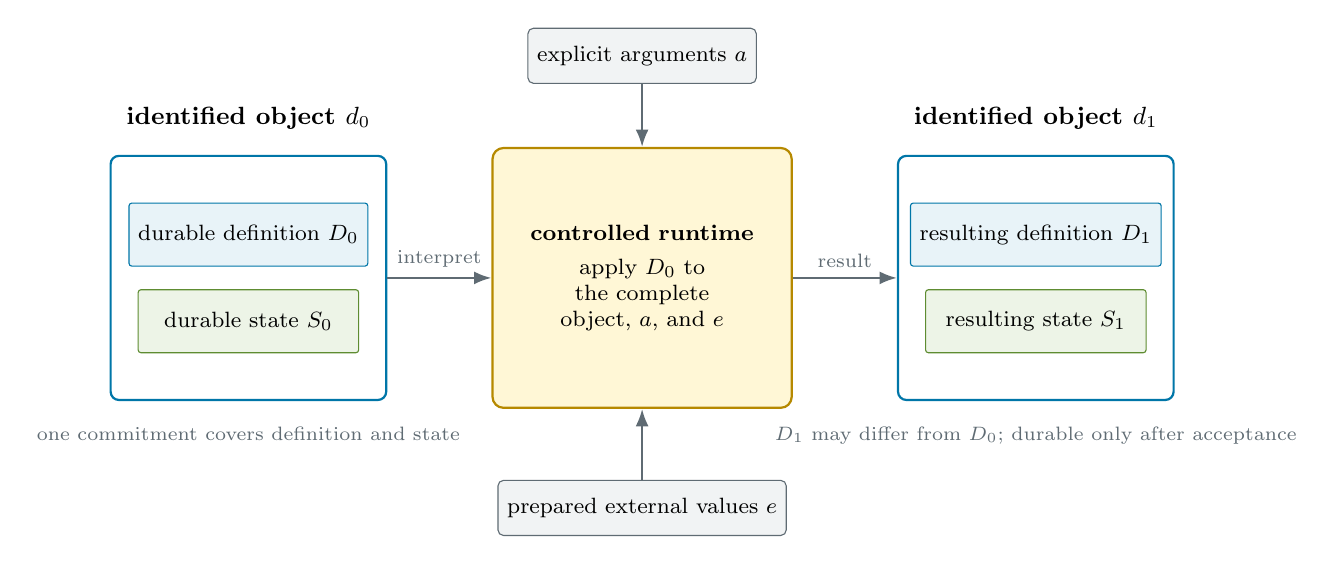
\begin{tikzpicture}[
  object/.style={draw=swblue, thick, rounded corners=3pt, fill=white,
                 minimum width=35mm, minimum height=31mm},
  part/.style={draw=swgray, rounded corners=1pt, minimum width=28mm,
               minimum height=8mm, align=center, font=\footnotesize},
  definition/.style={part, fill=swlightblue, draw=swblue},
  state/.style={part, fill=swlightgreen, draw=swgreen},
  runtime/.style={draw=swgold!85!black, thick, rounded corners=4pt,
                  fill=swlightgold, minimum width=38mm, minimum height=33mm,
                  text width=31mm, align=center, font=\footnotesize},
  input/.style={draw=swgray, rounded corners=2pt, fill=swlightgray,
                minimum width=28mm, minimum height=7mm,
                align=center, font=\footnotesize},
  arrow/.style={-{Latex[length=2.2mm]}, thick, draw=swgray},
  note/.style={font=\scriptsize, text=swgray, align=center},
]
  % Initial durable object.
  \node[object] (old) at (-5.0,0) {};
  \node[definition] (olddef) at (-5.0,0.55) {durable definition $D_0$};
  \node[state] (oldstate) at (-5.0,-0.55) {durable state $S_0$};
  \node[font=\small\bfseries, above=2mm of old.north] {identified object $d_0$};
  \node[note, below=2mm of old.south] {one commitment covers definition and state};

  % Controlled runtime and explicit input.
  \node[runtime] (eval) at (0,0) {\textbf{controlled runtime}\\[1mm]
                                  apply $D_0$ to the complete\\object, $a$, and $e$};
  \node[input, above=8mm of eval.north] (args) {explicit arguments $a$};
  \node[input, below=9mm of eval.south] (effects) {prepared external values $e$};
  \draw[arrow] (args) -- (eval);
  \draw[arrow] (effects) -- (eval);
  \draw[arrow] (old.east) -- node[above,note] {interpret} (eval.west);

  % Resulting durable object.
  \node[object] (new) at (5.0,0) {};
  \node[definition] (newdef) at (5.0,0.55) {resulting definition $D_1$};
  \node[state] (newstate) at (5.0,-0.55) {resulting state $S_1$};
  \node[font=\small\bfseries, above=2mm of new.north] {identified object $d_1$};
  \node[note, below=2mm of new.south] {$D_1$ may differ from $D_0$; durable only after acceptance};
  \draw[arrow] (eval.east) -- node[above,note] {result} (new.west);

\end{tikzpicture}
}
  \caption{Self-Encoding Object Transition}
  \label{fig:self-encoding-transition}
\end{figure}

Live mutation and durable mutation meet at explicit persistence: a method may update the live object's state, while the journal records the change after extracting the new node and storing it into its parent or root. Nested mutation rebuilds each containing object along the return path, keeping every predecessor available by digest and making the durable boundary visible in code. Objects compose through public protocols: deep reads traverse semantic boundaries, deep mutations rebuild ancestors, deep slicing and pruning ask each object to retain evidence appropriate to its layout, and deep merge restores compatible partial material under matching commitments. \Cref{tab:deep-operations} summarizes this implemented family. Portable definitions arrive from parties who may use different software and policy, so evaluation occurs inside a reduced environment: the s7 configuration removes broad filesystem, process, native-loading, network, random, and host-I/O authority; privileged orchestration obtains legitimate environmental values first and passes them as ordinary data; and authorization and explicit storage turn the candidate result into history.

\begin{table}[htbp]
  \centering
  \small
  \begin{tabularx}{\textwidth}{@{}>{\ttfamily\raggedright\arraybackslash}p{0.17\textwidth}>{\ttfamily\raggedright\arraybackslash}p{0.35\textwidth}X@{}}
\toprule
\normalfont\textbf{Operation} & \normalfont\textbf{Signature} & \textbf{Behavior} \\
\midrule
deep-get    & (deep-get object path) & Traverse nested public \texttt{get} methods and return the value at the path. \\
deep-set!   & (deep-set! object path value) & Set the terminal value and rebuild each containing object. \\
deep-slice! & (deep-slice! object path) & Retain evidence along the path while preserving the logical digest. \\
deep-prune! & (deep-prune! object path) & Remove evidence along the path, rebuilding parents or replacing exhausted children with stubs. \\
deep-merge! & (deep-merge! source target (path '())) & Merge digest-compatible evidence into the target or into the optional target path. \\
deep-copy!  & (deep-copy! object source-path target-path) & Read a value from one nested path and set it at another. \\
deep-call   & (deep-call object path callback) & Evaluate a callback against the selected object and return the callback result while leaving ancestors unchanged. \\
deep-call!  & (deep-call! object path callback) & Evaluate a callback, retain the mutated child node, and rebuild every ancestor. \\
\bottomrule
\end{tabularx}

  \caption{Deep Object Operations}
  \label{tab:deep-operations}
\end{table}

\section{A Controlled Semantic Web}

The project’s \texttt{standard.scm} object system demonstrates one way to grow semantics from a small evaluator: classes compile into portable nodes, methods operate through strict dispatch, trees and chains compose through public protocols, and ledgers place those objects into signed history. It provides one concrete reference architecture for portable objects, while other systems can participate by publishing durable protocols and preserving the structural invariants needed for slicing, persistence, and verification. This controlled foundation also opens two semantic surfaces: application-defined objects can carry scientific, institutional, and social structures as versioned concepts above the native runtime, while programmable queries can travel as inspectable code and execute against a fixed, authorized historical capability. Initial public queries should be read-only, metered, identified by digest, and able to return evidence for the data they touched. \WIP Installation, invocation, proof round trips, authorization, metering, and migration remain the acceptance tests for both facilities. Together they complete the progression from integrity to meaning, which Chapter~5 projects outward as a Web whose coordinates, identity, and trust begin from a selected journal. At network scale, control concentrates in three areas:

\begin{itemize}
  \item \textbf{Deterministic transition.} Successors derive from the starting object, definitions, explicit arguments, evaluator semantics, and controlled primitives; time, randomness, remote responses, and operator choices become prepared inputs. \WIP The current system-time procedures require removal, mediation, or recording.
  \item \textbf{Resource governance.} Evaluation needs bounds on time, allocation, recursion, reads, result size, and durable mutation, with atomic failure at a bound~\cite{Levy1995safe,Necula1997proof}. \WIP Object-specific budgets and capabilities would extend the current shared reduced environment.
  \item \textbf{Explicit evolution.} Public methods, return shapes, sentinels, and layouts form compatibility contracts, and migrations record the relation between old and successor definitions and state. \WIP Complete migration must cover authority, rollback, nested partial objects, validation, and long-term runtime compatibility.
\end{itemize}
\chapter{The Journal-Relative Web}
\label{sec:journal-web}
\label{sec:paths}
\label{sec:policy}

\section{Resources and Rooted Paths}

A resource is a leaf reached through path and object semantics. Its content may be uninterpreted bytes, an encoded expression, or another self-encoding structure. Resource identity has two complementary dimensions. A path gives the resource continuity within one selected journal-relative coordinate system, while a digest identifies the particular state resolved at that path.

Interpretation always begins from a root. A path without its root is incomplete in the same way that a relative URL is incomplete without a base. Traversal follows documented semantic boundaries rather than assuming one universal physical tree, so two objects may interpret the same path segment differently while still preserving an end-to-end integrity proof. Resolution itself proves neither existence, availability, principal identity, nor authority until the relevant structural and policy checks succeed.

\section{Plural Coordinates}

No global top-level registry is required. This follows traditions of linked local namespaces and self-certifying pathnames~\cite{Rivest1996sdsi,Mazieres1998path}. Each journal induces coordinates over the local and foreign state reachable from its root. Identical suffixes beneath two roots need not name the same resource, and a bridge segment records the relationship through which foreign state became reachable. A historical index additionally selects the committed head against which the rest of the path is resolved.

Traversal can end at a stub, an absent resource, an unreachable peer, private terminal state, or a policy denial. These outcomes have different meanings and should remain distinguishable to clients. Content identity, path continuity, human-readable naming, and principal identity are likewise separate concerns. Root-relative addressing complements content-bound and data-centric naming rather than replacing them~\cite{Haber1997secure,Kuhn2014trusty,Zhang2014named}.

Eliminating one mandatory naming authority moves work into root selection, discovery, route maintenance, and comparison among viewpoints. The network shown in \cref{fig:journal-relative-web} is therefore journal-relative: independently advancing histories are joined by sparse explicit relationships, with no enclosing global root from which every resource must descend.

\section{Web Projection}

Addressable network form and query-optimized operational form serve different purposes. The first favors independently identifiable resources, linking, selective transfer, citation, and plural ownership. The second favors application records, schemas, indices, transactions, compression, and local query performance. Neither is a universally superior physical representation; \cref{tab:data-forms} summarizes their complementary roles.

\begin{table}[htbp]
  \centering
  \small
  \begin{tabularx}{\textwidth}{@{}p{0.18\textwidth}XX@{}}
\toprule
\textbf{Aspect} & \textbf{Addressable Network Form} & \textbf{Query-Optimized Operational Form} \\
\midrule
Primary unit & Independently identified resource and relationship & Application record, row, object, index, or transaction \\
Identity & Root-relative path plus resolved state commitment & Application key interpreted within one operational system \\
Strengths & Linking, citation, selective transfer, plural ownership, and historical reference & Locality, transactions, compression, indexing, and efficient bounded queries \\
History & Durable resource states and cross-history relationships are first-class & Commonly application-defined, compacted, or maintained in separate logs \\
Typical costs & Traversal, synchronization, repeated metadata, and derived indexing & Provider dependence, schema coupling, and application-specific portability \\
Architectural role & Shared network projection and durable evidence & Load-bearing operations and rebuildable derived views \\
\bottomrule
\end{tabularx}

  \caption{Complementary Data Forms}
  \label{tab:data-forms}
\end{table}

A Web projection lets an operational system remain load-bearing while selected state receives a durable addressable form. The projection must define resource boundaries, deterministic encodings, path conventions, progress manifests, and the semantics of correction, privacy, deletion, and replay. It does not automatically inherit every invariant of its source. Transaction boundaries, relational constraints, and mutable deletion policies may require explicit representation in the projected history.

Adoption can therefore proceed incrementally. An asynchronous projection first supplies an audit path. As clients, authorization, query facilities, and monitoring mature, selected projected resources may become load-bearing. Observable cursors and deterministic correction records make lag and divergence explicit, but coexistence still costs synchronization, reconciliation, and duplicated storage. \WIP General projection contracts for dynamic applications, privacy-sensitive records, correction, and bidirectional synchronization remain unsettled.

\section{Historical Identity and Keys}

\WIP A remote principal becomes meaningful only when the receiving journal can resolve the origin through its own bridge graph to a current public interface key. A synchronized descriptor binds the remote journal's name, stable root key, current interface key, canonical endpoints, head, and historical context. Unverified information endpoints and private configuration may cache those facts for convenience, but they cannot override the signed state.

The root key signs journal heads and is a pinned, non-rotating trust anchor in the initial design. Interface keys sign federated invocations and may change after their replacements appear in root-signed heads synchronized through the bridge graph. A compiled return proof reveals the exact origin checkpoint and interface key that the terminal can verify. The origin can use that retained key or complete its final local proof segment to a newer key authorized by a later root-signed head.

A stored head provides reverse cryptographic reachability even when its journal cannot accept inbound transport. Cryptographic reachability, network reachability, and responsibility for initiating synchronization are therefore distinct. Reciprocal heads, descriptors, continuity evidence, and route proofs form a public control plane; none grants authority over private application state.

\section{Federated Route Establishment}

\WIP A private federated invocation begins with one public multi-hop request and response that compile two different proofs. Each proof is rooted in the current state of the endpoint that will consume it. For an origin A and terminal B, the forward leg constructs A's proof of B. A begins with the exact adjacent-journal checkpoint stored in A's current head. Every intermediary proves continuity from the checkpoint it was actually given to its current head, then contributes the next nested checkpoint stored there. B completes the proof to its current root identity, interface key, head, descriptor, and canonical endpoint.

The return leg starts from B's own current head and follows the reverse checkpoints in the same manner. When the response reaches A, A completes the final segment to the interface key it will use to sign. This endpoint-relative construction prevents an upstream journal from guessing what a later participant has synchronized. Every link consists of committed Merkle inclusion and signed chain continuity; no live intermediary attestation is treated as though it had already been committed into the terminal's graph.

The resulting B-relative source proof is mandatory on the direct invocation. Beginning from its own current head, B can verify the proof, resolve the exact A interface key selected by it, verify A's signature, construct the receiver-relative principal, authorize the function, and execute it in one pass. This realizes a more abstract verifiable-chain idea: identity is established through a connected path that the relying endpoint can verify from its own state and through which evidence is traced in both directions~\cite{dinh2025identity}.

After the public handshake, A sends the signed function, arguments, private paths, and values directly to B over HTTPS. Intermediate journals handle only public proof and discovery material; they neither relay nor observe the private call. The design consequently requires the terminal to be reachable and deliberately excludes onion routing, encrypted offline relay, and offline delivery of private invocations. The origin signature binds the complete semantic route, terminal audience, explicit identity, function, and arguments. Local credentials and private signing keys remain inside the origin journal boundary.

\Cref{fig:federated-invocation} separates the compiled public route from the direct final mile. The self-contained proof removes the need for a terminal route cache, compact terminal-issued receipt, or second reverse traversal. \WIP Exact proof serialization, bridge-alias translation, endpoint and head races, retry behavior, and terminal response binding remain to be specified.

\begin{figure}[htbp]
  \centering
  \resizebox{0.88\textwidth}{!}{% Public routing follows exact nested journal objects already committed beneath
% the origin head.  The private invocation then bypasses the intermediary.
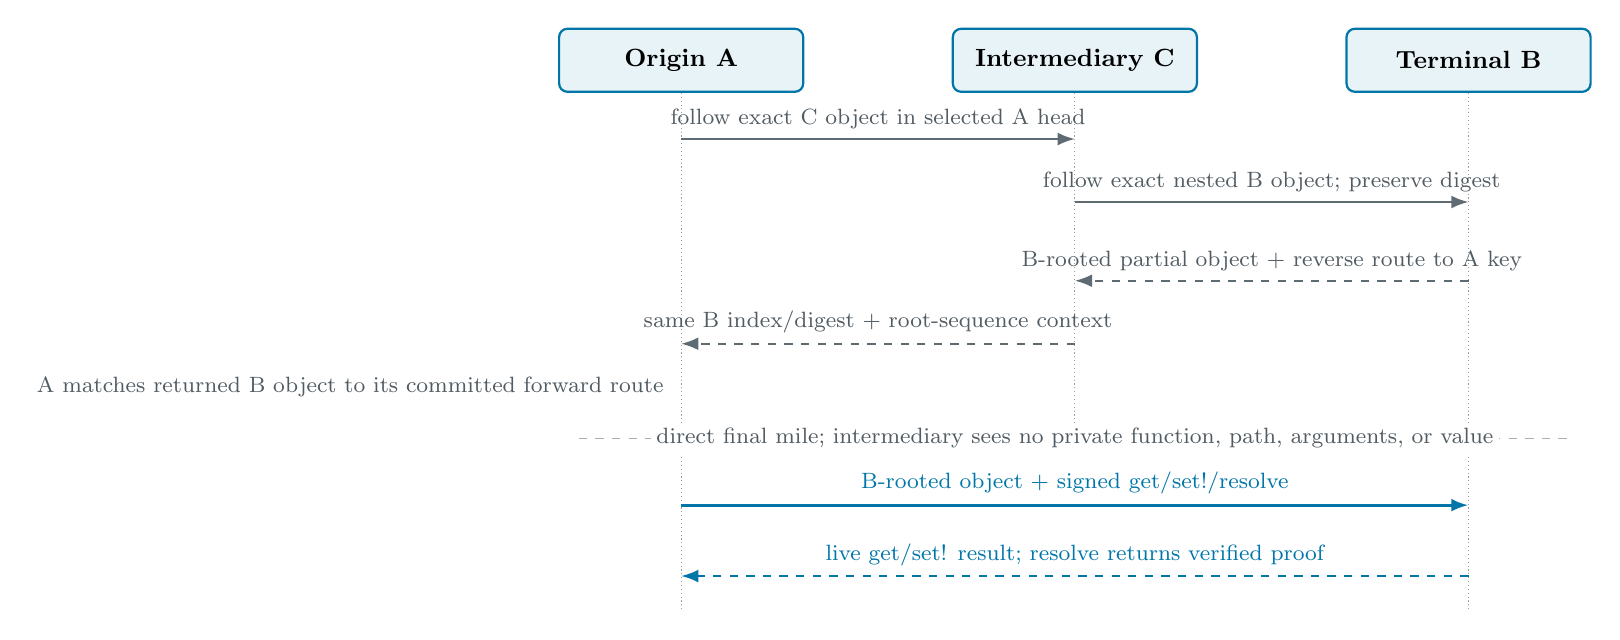
\begin{tikzpicture}[
  participant/.style={draw=swblue, thick, rounded corners=3pt, fill=swlightblue,
                      minimum width=31mm, minimum height=8mm,
                      font=\small\bfseries, align=center},
  lifeline/.style={draw=swgray!65, densely dotted},
  msg/.style={-{Latex[length=2.2mm]}, thick, draw=swgray},
  return/.style={msg, dashed},
  direct/.style={msg, draw=swblue, very thick},
  note/.style={font=\footnotesize, text=swgray!85!black, align=center},
]
  \node[participant] (a) at (-5.0,0) {Origin A};
  \node[participant] (c) at (0,0) {Intermediary C};
  \node[participant] (b) at (5.0,0) {Terminal B};
  \draw[lifeline] (a.south) -- (-5.0,-7.0);
  \draw[lifeline] (c.south) -- (0,-4.9);
  \draw[lifeline] (b.south) -- (5.0,-7.0);

  \draw[msg] (-5.0,-1.0) -- node[above,note]
    {follow exact C object in selected A head} (0,-1.0);
  \draw[msg] (0,-1.8) -- node[above,note]
    {follow exact nested B object; preserve digest} (5.0,-1.8);

  \draw[return] (5.0,-2.8) -- node[above,note]
    {B-rooted partial object + reverse route to A key} (0,-2.8);
  \draw[return] (0,-3.6) -- node[above,note]
    {same B index/digest + root-sequence context} (-5.0,-3.6);
  \node[note, anchor=east] at (-5.1,-4.15)
    {A matches returned B object to its committed forward route};

  \draw[swgray!55, dashed] (-6.3,-4.8) -- (6.3,-4.8);
  \node[note, fill=white, inner sep=2pt] at (0,-4.8)
    {direct final mile; intermediary sees no private function, path, arguments, or value};

  \draw[direct] (-5.0,-5.65) -- node[above,note, text=swblue]
    {B-rooted object + signed get/set!/resolve} (5.0,-5.65);
  \draw[return, draw=swblue] (5.0,-6.55) -- node[above,note, text=swblue]
    {live get/set! result; resolve returns verified proof} (-5.0,-6.55);
\end{tikzpicture}
}
  \caption{Compiled Route Proof and Invocation}
  \label{fig:federated-invocation}
\end{figure}

\section{Journal Boundary and Authorization}

External requests enter through a controlled journal interface responsible for authentication, authorization, argument normalization, route preparation, batching, and explicit persistence. Network fetches and service credentials remain outside deterministic object methods. Administration over code, roots, bridges, secrets, and policy remains local even when ordinary resource operations become federated.

\WIP Invocation identity is explicit and scalar. It identifies the originating journal, one user locally authenticated by that journal, or a public caller. Omission is invalid and can never imply privileged journal identity. At the receiver, the verified route and scalar identity combine into the canonical receiver-relative principal path used by authorization.

When the scalar denotes a local user, the origin attests that it authenticated that user through its own session or token system. The terminal does not validate the remote password or session. It first authenticates the origin journal and proof, then decides what authority to grant the narrower user attestation. Every terminal operation and every dynamically discovered read requires an explicit local rule; bridge reachability, signatures, and structural integrity are not permission.

Prefix rules express ordinary ownership efficiently, but they may not capture object methods, callbacks, or effects spanning several paths. Principal authentication should also remain distinct from verifiable-credential infrastructure~\cite{Sedlmeir2021digital}. \WIP The signed sender flow, authenticated response envelope, arbitrary object methods, links, and programmable reads still require end-to-end inspection.

\section{Replay and Mutation}

Federation does not promise exactly-once execution. It maintains no generic durable request-ID table, nonce protocol, timestamp window, or replay cache, so a valid signed invocation may be replayed. Reads, route proofs, and head synchronization must therefore be idempotent, with ordinary rate and resource controls limiting repeated expensive work.

A mutation must either be naturally replay-safe, explicitly permit repetition, or carry a signed operation-specific precondition such as an expected revision or state digest. A successful guarded mutation advances that state, so replaying the old signed request fails its precondition rather than restoring stale data. Operations with irreversible external effects need stronger domain-specific idempotency and should not become federated merely because their request can be signed. \WIP The first federated mutation set and the precondition semantics for each function remain to be selected.

\section{Links and Discovery}

\WIP A first-class link identifies a target through an explicit root and relationship context and states whether resolution is current or historical. The integrity of the link and the integrity of the target are separate. Traversal must preserve route and authority boundaries and distinguish a broken link from private, unauthorized, malformed, unavailable, or internally inconsistent state. Unrestricted traversal also creates privacy, denial-of-service, and confused-deputy risks.

Discovery finds candidate journals, resources, endpoints, and routes through social exchange, indices, descriptors, existing bridges, or out-of-band knowledge. A discovered candidate does not thereby become accepted or authoritative. Candidates may be stale, mutually inconsistent, or malicious; local policy decides which relationships to create and which routes to follow. Endpoint and interface-key changes require root-signed historical continuity because discovery metadata evolves. Root-key recovery and rotation remain deferred.

\section{Transparent Clients and Adapters}

The primary interaction model is ordinary data rather than proof ceremony. Clients read and write resources, invoke objects, follow links, and resolve history. A specialized local client chooses roots and historical context, fetches and merges evidence, enforces policy, reports meaningful failure distinctions, and applies retention intent beneath those operations.

Cryptography narrows dependence on remote operators but does not eliminate the local trusted computing base. Users still depend on their client, evaluator, operating system, and key store. Gateways, filesystems, browsers, inspection tools, and projection workers are replaceable adapters over common resource and history semantics, yet any adapter can hide richer behavior or misrepresent a result and therefore remains within a client or service trust boundary.

Application protocols and provenance vocabularies belong above the generic structures~\cite{Moreau2010open,Groth2010anatomy,BernersLee2001semantic}. \WIP Native browsers and computational views should make routine verification unobtrusive while preserving explicit audit and debugging views for specialists.

\chapter{Application Sketches}
\label{sec:applications}
\label{sec:worked-example}

The following sketches test the architecture against domains with different institutions, retention horizons, and consequences. They are not claims of completed applications. Each illustrates how independent histories, selected projection, and local policy can supply value without requiring one shared operational database.

\section{Supply Chain Traceability}

Manufacturers, carriers, inspectors, and buyers can retain their own operational histories while linking selected records across changes of custody. A recipient can preserve the component record it received, associated certificates and inspection evidence, and the exact state against which its decision was made. The evidence remains interpretable even if the originating organization's current database later changes.

This arrangement parallels the NCCoE manufacturing traceability model~\cite{Stouffer2022traceability}. Secure-provenance research likewise treats integrity and controlled disclosure as essential when records cross organizational boundaries~\cite{Hasan2009provenance}. The journal-relative form adds independently retained history and explicit cross-history relationships without forcing every participant into one application database.

The result is evidence of recorded pedigree, not proof of physical reality. Binding a record to a physical component still requires sensors, identifiers, inspections, procedures, and institutional accountability. The system can preserve disagreements among those sources; it cannot decide which physical-world assertion is true.

\section{Persistent Web Archives}

Web resources can be projected into independently operated journals as durable, historically versioned state. Multiple archives may preserve overlapping portions of a site's history and entangle their own histories rather than depend on one archival operator. Root-relative links can identify both the continuing resource lineage and a particular captured state while the ordinary source system continues serving current traffic.

This model separates operational publication from long-term evidence. An existing static site, content-management system, or database may remain load-bearing while an asynchronous projection adds integrity-verifiable history. If native clients later mature, selected projected resources may assume a larger operational role without requiring an all-at-once migration.

Long-term storage research warns that unlikely failures and cryptographic aging become ordinary over decades~\cite{Chun2009tiered}. Archives therefore still need capture-fidelity, privacy, legal-erasure, malicious-content, media-renewal, retention, and migration policies. Historical integrity makes alteration detectable relative to retained commitments; it does not operate the archive indefinitely.

\section{Portable Identity Anchors}

A person can establish a stable path beneath a selected well-known root and use it to identify a current profile hosted by a replaceable journal. Moving the profile then becomes a historical transition rather than the abandonment of every established reference. Observers can resolve the old relationship, inspect the later redirecting state, and decide whether the transition satisfies their own trust policy.

Historic name trails provide a close precedent: obsolete provider-controlled names can lead to later user-directed identifiers while preserving the evidence of transition~\cite{Maniatis2003hints}. Journal-relative history extends this pattern to richer state and reciprocal relationships.

Portability reduces dependence on one host, but it does not remove the need for anchor governance, key recovery, impersonation defenses, endpoint discovery, privacy, or continued availability. A stable path is useful only to observers who accept its root and can obtain enough history to verify the transition.

\section{Agent Reputation Discovery}

A user can choose journals or communities as starting roots and discover reporting agents through explicit relationships instead of accepting one platform ranking. An agent's reports, cited sources, corrections, and later outcomes become locally resolvable evidence for reputation judgments. Different communities can retain different evidence and reach different conclusions without collapsing those judgments into a universal score.

Secure per-node logs and deterministic replay offer a related model for observable accountability~\cite{Haeberlen2007peerreview}. The Synchronic Web adds partially retained resource history and relationship-relative discovery, allowing the evidence used by one evaluation to remain identifiable after the ranking or agent changes.

Durable history cannot eliminate Sybil identities, collusion, compromised keys, selective reporting, or repeated falsehoods. It can make the basis of local judgment inspectable and make later correction distinguishable from retrospective rewriting. Institutions and users still decide which roots, witnesses, and evaluation rules deserve weight.

\section{Common Pattern}

Each sketch begins with independently administered operational state. Selected resources receive stable root-relative coordinates, local commitments preserve successive states, and explicit relationships connect histories across institutions. Partial evidence permits selective retention, self-encoding structure keeps durable interpretation associated with the state, and local policy decides which remote identities and operations carry authority.

The recurring value is not universal agreement. It is the ability to retain and compare evidence across institutions and time without requiring those institutions to share one operator, schema, or global sequence. The same architecture also preserves the limits of that evidence: availability, physical binding, social trust, and policy remain external obligations.

\chapter{Related Work and Lineage}
\label{sec:related-work}

\section{Terminology}

The literature ordinarily uses \emph{authenticated data structure} for a structure whose answers can be checked against a commitment. This paper usually says \emph{integrity-verifiable} because it reserves authentication for claims about identity, origin, and authority. The distinction separates three propositions that are often conflated: a value is consistent with a digest, a key signed that digest, and a locally meaningful principal is authorized to perform an operation. Established terminology is retained when naming a cited field or construction.

\section{Integrity and Entangled History}

Cryptographic timestamping and persistent authenticated dictionaries establish committed succession and historical queries~\cite{Haber1991timestamp,Anagnostopoulos2001persistent}. General models and generic programming techniques extend authenticated data structures beyond one fixed tree, while compact Merkle multiproofs and tamper-evident logs reduce or organize the evidence retained for verification~\cite{Martel2004general,Miller2014authenticated,Ramabaja2020compact,Crosby2009efficient}. Certificate, key, and software transparency apply related structures to constrain equivocation by particular authorities~\cite{Laurie2014certificate,Melara2015coniks,Nikitin2017chainiac}. A journal history can serve such an accountability role, but it also carries general path-addressable application state.

Maniatis and Baker's secure timeline entanglement is the closest direct precedent for bridge-composed history~\cite{Maniatis2002timeline}. Mutually distrustful services import signed foreign timeline threads into later authenticators, producing temporal mappings, incorporation receipts, and evidence that can survive the originating service. The Synchronic Web makes no novelty claim for this cross-history mechanism. It combines entanglement with proof-preserving partial possession, self-encoding structures, root-relative resources, and sparse relationships rather than the all-to-all entangled service set analyzed in Timeweave.

Timeline evidence establishes a branch, not its uniqueness. PeerReview adds attributable logs and deterministic replay for observable distributed behavior~\cite{Haeberlen2007peerreview}. Transparency overlays and gossip provide a more general way to expose inconsistent views without assuming that a signature prevents them~\cite{Chase2016transparency}. These precedents ground the paper's explicit separation between fork evidence and fork prevention.

\section{Storage, Provenance, and Preservation}

Untrusted-storage systems demonstrate how clients can detect tampering and inconsistent views without assuming an honest server~\cite{Li2004secure,Mahajan2010depot,Kim2015caelus}. The Synchronic Web shares that distrust boundary but does not require unrelated journals to converge on one stored state. Database provenance distinguishes why- and where-provenance, while Web provenance work developed process and evidence models~\cite{Buneman2001why,Moreau2010foundations,Moreau2010open}. W3C PROV subsequently standardized a domain-independent model of entities, activities, agents, derivations, and responsibility for interoperable exchange~\cite{Moreau2013prov}. Nanopublications apply a compact assertion-and-provenance form to scientific communication~\cite{Groth2010anatomy}, and secure provenance adds integrity and confidentiality for provenance crossing untrusted environments~\cite{Hasan2009provenance}. These vocabularies can inhabit journal resources without becoming the substrate's mandatory ontology.

IPFS and Trusty URIs use content-derived identifiers, while secure names and self-certifying pathnames bind names or paths to verifiable material~\cite{Benet2014ipfs,Kuhn2014trusty,Haber1997secure,Mazieres1998path}. Merkle-CRDTs use Merkle DAGs as transport and persistence for convergent replicated data, Named Data Networking makes named data central to retrieval, and LOCKSS uses peer-to-peer replication and auditing for preservation~\cite{Sanjuan2020merkle,Zhang2014named,Maniatis2005lockss}. The Synchronic Web instead joins partial structure, durable interpretation, and independent historical viewpoints in one resource model. Tiered long-term fault tolerance further emphasizes that rare threshold failures and cryptographic aging become likely over archival time scales~\cite{Chun2009tiered}; logical identity still requires renewal and operational preservation.

\section{Addressing and Decentralized Webs}

Canonical Web architecture separates resource identification, representations of resource state, and agent interaction, while URI syntax resolves relative references against a base~\cite{Jacobs2004webarch,BernersLee2005uri}. Synchronic Web paths borrow the rooted-resolution intuition but are not globally scoped URIs. Memento adds HTTP datetime negotiation and TimeMaps for prior resource states~\cite{VanDeSompel2013memento}; journal history instead makes temporal resolution recursive within its resource model. Historic name trails follow changes in personal online identifiers and provide a direct precedent for portable identity anchors~\cite{Maniatis2003hints}.

SDSI provides linked local namespaces, while SPKI/SDSI certificate-chain discovery constructs proofs of naming and delegated authority for evaluation against a relying party's access policy~\cite{Rivest1996sdsi,Clarke2001chain}. Decentralized trust management similarly separates presented credentials from local policy evaluation~\cite{Blaze1996trust}. Earlier Synchronic Web identity work describes verifiable chains as intermediary links that a verifier can trace to an anchor and back~\cite{dinh2025identity}. The compiled endpoint-relative route proof in this paper gives that abstract connectedness a construction rooted in the relying journal's actual state.

Local-first software centers authoritative local copies and user ownership, while Solid places user-controlled data in stores that applications can access independently~\cite{Kleppmann2019local,Mansour2016solid}. Webstrates persists and synchronizes mutable DOM state, including code, whereas the AT Protocol combines signed per-user repositories with decentralized service providers and account portability~\cite{Klokmose2015webstrates,Kleppmann2024bluesky}. Data spaces address governance among organizations, and the Semantic Web pursues machine-interpretable relationships across Web resources~\cite{Otto2019designing,BernersLee2001semantic}. The Synchronic Web adds integrity-preserving history, partial possession, and self-encoding interpretation beneath application interfaces; it does not claim that cryptography supplies moderation, governance, semantics, or usable institutions.

\section{Persistent and Distributed Semantics}

Orthogonal persistence makes values persist without type-specific storage code, while tierless languages reduce representation boundaries among application layers~\cite{Atkinson1983approach,Cooper2007links}. Emerald supports mobile objects in a distributed language; Argus structures distributed programs around encapsulated guardians and atomic actions~\cite{Raj1991emerald,Liskov1988distributed}. Safe interpreters restrict ambient authority at runtime, whereas proof-carrying code supplies statically checkable evidence of prescribed properties~\cite{Levy1995safe,Necula1997proof}. Self-encoding objects combine durable behavior and state but retain a local evaluator and policy boundary.

Ethereum fixes replicated transaction execution under a global ledger, whereas Hyperledger Fabric combines permissioned governance with endorsement, ordering, and validation~\cite{Wood2014ethereum,Androulaki2018hyperledger}; journal evaluation remains locally administered. Tuple spaces provide shared associative environments~\cite{Gelernter1985generative}. Bayou addresses weak connectivity and reconciliation, Dynamo prioritizes availability under failures, and CRDTs define convergent replicated data types~\cite{Terry1995managing,DeCandia2007dynamo,Shapiro2011conflict}. The CALM line characterizes when monotonic programs can avoid coordination~\cite{Hellerstein2020keeping}, while Merkle search trees organize state-based CRDT exchange in open networks~\cite{Auvolat2019merkle}. Historical composition preserves independent viewpoints without promising convergence.

\section{Agents and the Proposed Combination}

Retrieval-augmented generation supplies models with external documents; Generative Agents stores experience streams and higher-level reflections; AriGraph integrates semantic and episodic memory in a graph; and HippoRAG builds a long-term retrieval index~\cite{Lewis2020retrieval,Park2023generative,Anokhin2025arigraph,Gu2024hipporag}. Agent-oriented programming and communication languages supply a longer lineage for explicit agent state, intention, and interaction~\cite{Shoham1993agent,Finin1994kqml}. These systems motivate a demanding consumer of history, but the Synchronic Web is not an agent framework.

Verifiable-credential systems foreground issuer, holder, verifier, claim, and proof roles~\cite{Sedlmeir2021digital}. The Synchronic Web instead puts ordinary resource interaction first and asks clients to conceal routine verification beneath reads, writes, links, and invocations. Credentials may be represented as application resources, but their ceremony does not define every interaction.

Clear precedents exist for every individual ingredient. The proposed contribution is the architectural composition in which self-encoding structures retain identity under partial possession, independently rooted histories become entangled, journal-relative paths turn those histories into a plural Web, and clients hide routine proof machinery beneath ordinary operations. Composition alone is not proof of practical value. Implementation inspection, usability work, operational evidence, and continued literature comparison remain necessary before any broader novelty claim.

\chapter{Discussion and Conclusion}
\label{sec:assessment}
\label{sec:properties}
\label{sec:tradeoffs}
\label{sec:conclusion}

\section{Bounded Guarantees}

The architecture provides bounded properties relative to explicit commitments, evaluator semantics, retained evidence, and local policy. It does not make unconditional security claims. \Cref{tab:assurance-matrix} summarizes the principal mechanisms in the same form used throughout the paper: the property obtained, the property not obtained, and the burden displaced elsewhere.

\begin{table}[htbp]
  \centering
  \small
  \begin{tabularx}{\textwidth}{@{}>{\raggedright\arraybackslash}p{0.18\textwidth}>{\raggedright\arraybackslash}X>{\raggedright\arraybackslash}X@{}}
\toprule
\textbf{Mechanism} & \textbf{Provides} & \textbf{Limits and Displaced Burden} \\
\midrule
Integrity structure & Consistency with an accepted commitment & Does not establish origin, authority, truth, or availability; requires commitment acquisition and correct verification. \\
Partial structure & Selected evidence tied to one complete-state identity & Does not reveal hidden content or prove completeness or future retrieval; requires proof metadata, disclosure policy, and retention. \\
History & Detectable state succession and prior-state identity & Does not ensure one branch or physical preservation; requires storage, key continuity, migration, and witness comparison. \\
Self-encoding structure & Durable association between state and interpretation & Does not ensure safety, termination, compatibility, or correctness; requires confinement, metering, documentation, and migration. \\
Entanglement & Cross-history ordering and survivable incorporation receipts & Does not provide consensus, fork prevention, trust, or authority; requires synchronization, incorporation, witnesses, and policy. \\
Federated route & Mutual endpoint identity and a direct authenticated final mile & Does not provide authorization, anonymity, offline relay, or exactly-once execution; requires proof freshness, terminal reachability, local rules, and replay-safe mutation. \\
Rooted paths & Resource continuity from a selected viewpoint & Do not supply universal naming or discovery; require root choice, route maintenance, and indexing. \\
\bottomrule
\end{tabularx}

  \caption{Architectural Assurance Boundaries}
  \label{tab:assurance-matrix}
\end{table}

\section{Explicit Non-Properties}

Integrity is not availability. A valid digest may identify data that no reachable participant still possesses, so preservation requires replication and operational commitment~\cite{DeCandia2007dynamo,Maniatis2005lockss}. Signatures likewise establish branches rather than one unique global view. Witness comparison and transparency overlays can expose forks, but bridges do not prevent a dishonest journal from presenting them~\cite{Maniatis2002timeline,Chase2016transparency}. Unrelated journals need not converge and share no mandatory consensus.

A bridge, digest, signature, or path does not imply trust, endorsement, authorization, or semantic truth. Partial structure is not confidentiality; private final-mile communication requires access control and authenticated secure transport, normally TLS/HTTPS in secure deployments, with additional encryption where the application demands it. Federation supplies neither anonymity, onion routing, offline private relay, nor generic exactly-once execution.

Self-encoding definitions are not guaranteed to terminate, remain compatible, or behave correctly. Root-key recovery is especially consequential: the initial design cannot rotate a lost or compromised trust anchor without an out-of-band decision that established peers do not yet know how to authenticate. Discovery, moderation, governance, human-readable naming, and legal erasure remain institutional and application concerns. The architecture can preserve evidence relevant to those decisions, but it cannot make the decisions socially legitimate.

\section{Costs and Displaced Burdens}

Integrity adds hashing, persisted handles, proof paths, and traversal beyond the cost of storing raw bytes. Historical retention multiplies state even when immutable sharing reduces duplication. Partial possession saves content storage but still retains ancestor paths, stubs, digests, and serialization metadata. Fine-grained resource addressability improves citation and selective transfer while increasing path depth, object overhead, and reliance on derived indices.

Self-encoding interpretation adds evaluation, method dispatch, confinement, metering, debugging, versioning, and migration relative to inert data. Root plurality removes a mandatory naming authority but requires local key management, endpoint continuity, route comparison, and discovery. Federated calls add public proof compilation, freshness concerns, terminal reachability, direct transport, terminal authorization, and operation-specific replay safety.

Cross-journal workflows still require coordination when applications demand deadlines, exclusivity, payment, settlement, or globally unique allocation. Decentralization changes who may decide and who must operate the infrastructure; it does not make preservation or coordination free.

\section{Scale and Assurance Work}

\WIP Evaluation should measure history growth, proof size, bridge-graph traversal, bulk projection, self-encoding objects, and programmable queries under explicit workloads and resource budgets. Derived relational, search, and semantic indices may accelerate reads as long as they remain rebuildable views rather than untracked semantic authorities. Route proofs need bounded depth, cycle detection, proof-size limits, freshness rules, and reuse of verified evidence. Bulk projection needs batching, compaction, and observable progress.

\WIP Formal models should distinguish logical digest from persisted handle, root advancement from mutation, partial possession from absence, strict evaluation from durable acceptance, and bridge acceptance from historical incorporation. Core invariants include preservation of digest under slice, prune, serialization, and compatible merge; atomic failure of strict evaluation; predecessor continuity; and local authorization despite remote historical reachability.

Property tests, model checking, and source inspection must connect the declarative claims in this paper to active implementations. The draft should not become a final specification merely because its conceptual pieces are coherent.

\section{When Simpler Systems Suffice}

An ordinary database is preferable when one operator, current state, and efficient local queries are sufficient. Signed documents are simpler when the only requirement is publisher authentication of complete immutable payloads. Content-addressed storage is sufficient for immutable retrieval by digest, and a transparency log is better matched to public accountability for one authority.

CRDTs and conventional distributed services are appropriate when replicas should converge on one application state. A globally ordered ledger is appropriate when participants require a shared transaction order and accept the governance and execution costs of consensus. The Synchronic Web is justified only where independent roots, partial possession, self-encoding interpretation, and entangled history are jointly consequential. Using the complete architecture where one of these simpler models suffices would add burden without corresponding value.

\section{Return to Human Agency}

The architectural mechanisms return to the human problem with which the paper began. Durable historical grounding can support self-sovereign agency, decentralized reputation, and collective struggles over trustworthy information. People and communities can preserve their own roots while referring to evidence retained by others, without requiring one universal platform or owner.

This possibility still depends on usable clients, durable institutions, preservation work, and legitimate policy. Cryptographic evidence cannot replace social judgment; it can make the record on which judgment operates harder to rewrite silently. Agents increase both the utility of persistent history and the harm of opaque or manipulated context, but they remain participants and instruments rather than the final beneficiaries.

\section{Final Architectural Claim}

The Synchronic Web combines integrity-protected partial state, self-encoding structure, timeline-entangled history, and journal-relative resources under plural local authority. Timeline entanglement supplies the foundational cross-history principle~\cite{Maniatis2002timeline}. The larger claim is that this principle becomes a Web substrate when independent histories carry ordinary resources together with the durable definitions needed to interpret them.

The claim is conditional. Integrity depends on an accepted commitment and a correct verifier. Interpretation depends on a compatible controlled runtime. Availability depends on retention and replication. Remote authority depends on historical authentication and terminal-local authorization. Human value depends on institutions and clients that use those mechanisms responsibly.

The paper should remain a draft until authorization, compiled route proofs and response binding, mutation preconditions, incorporation receipts, first-class links, programmable queries, application-defined objects, metering, migration, and key lifecycle survive implementation inspection and testing. If those mechanisms hold, the resulting architecture offers neither a global database nor a universal source of truth, but a more modest and potentially more durable foundation: a Web in which plural histories can remain independently owned, partially known, mutually referential, and verifiable across time.

\section*{Glossary}
\label{sec:glossary}
\addcontentsline{toc}{section}{Glossary}

Reference definitions for recurring terms introduced throughout the paper.

\begin{description}[style=nextline]
  \item[Authentication]
    Verification of an asserted identity, origin, or authority through evidence such as credentials and signatures. Merkle integrity supplies the complementary structural check against a commitment.

  \item[Authorization]
    A policy decision determining whether a principal may perform an operation. In current federation, terminal-local rules grant remote principals path-scoped \texttt{get}, \texttt{set!}, and \texttt{resolve} permissions; administrators remain local principals.

  \item[Bridge]
    A reciprocal signed-head-retention relationship through which each journal preserves a verified head for the other. Reciprocity provides identity and history reachability, while terminal policy independently grants application-data authority.

  \item[Digest]
    A cryptographic hash derived from a node or larger structure and used as its integrity identifier.

  \item[Historical cursor]
    The independently selected origin and per-hop indexes used only by \texttt{resolve}. A canonical public journal-relative path interleaves these indexes with directional aliases; the Interface separates that path into the current route used for authentication and endpoint context and the historical cursor used to select committed content.

  \item[History]
    Used in its ordinary broad sense for prior states and changes. Concrete chains, heads, and receipts represent history using ordinary Synchronic Web structures.

  \item[Integrity]
    The property that modification can be detected relative to a known commitment. Authentication and authorization supply the associated claims about identity, origin, and authority.

  \item[Journal]
    The software an entity runs together with all data persisted on it. A journal supplies the root from which that entity views the Synchronic Web and is analogous to a site or origin on the conventional Web.

  \item[Journal identity]
    A stable commitment formed from a domain-separated random nonce and bound by bridges, preapprovals, and invocation audiences. Active signing keys may evolve beneath this identity through predecessor-authorized transitions.

  \item[Key-index]
    The terminal-local history index whose committed bridge state authenticated a remote interface key. Authorization may constrain this index relative to the terminal's current history.

  \item[Merge]
    To combine compatible partial structures whose integrity relationships agree.

  \item[Node]
    A generic term whose meaning follows from context. It may denote a node in the integrity-verifiable data-structure DAG or an entity in the graph of journals and relationships.

  \item[Object]
    A durable structure that couples executable behavior with state. Its documented protocol determines how the state is read, transformed, and represented; its internal layout remains implementation-specific.

  \item[Origin-local pin]
    Retention of verified remote proof material in the originating journal under the full origin-relative historical path. It follows a federated \texttt{resolve} and mutates the origin's retention state.

  \item[Path]
    A sequence interpreted from a selected journal root to address a resource or intermediate structure. A canonical federated path interleaves optional historical indexes with directional aliases before the terminal namespace and local path. Like a relative URL, its meaning is completed by a starting root.

  \item[Prune]
    To remove retained material while preserving the integrity relationships needed to identify the larger structure.

  \item[Record]
    Any snippet of data stored on a journal or transmitted between journals. The term is intentionally fluid across object shapes, historical entries, and storage units.

  \item[Resource]
    A path-addressed value or object in a journal-relative view. Its low-level representation may be a leaf or a larger self-encoding structure.

  \item[Root]
    A distinguished reference from which persisted structure is reached and interpreted. Unless otherwise qualified, a journal root is also the starting point for paths in that journal's view.

  \item[Root commitment]
    A digest or integrity reference accepted as the fixed point against which a structure is verified. Additional evidence is required to establish who created, supplied, or endorsed it.

  \item[Slice]
    A proof-preserving partial structure retaining the material required for selected paths while replacing unrelated material with stubs.

  \item[State]
    Used in its ordinary broad sense for the condition or contents of a system, structure, object, or resource at a relevant point or context.

  \item[Step]
    A discrete journal transition that turns staged changes into a new historically resolvable state.

  \item[Stub]
    A representation that retains the digest of unavailable, undisclosed, or intentionally pruned structure while omitting its contents. A stub represents unknown structure; null represents empty structure.

  \item[Stump]
    The low-level persisted node form used to represent a stub. It stores a retained logical digest under a distinct local node handle.

  \item[Synchronic Web]
    The network, data structure, computational medium, and protocol family formed when independently rooted journals make resources and histories reachable through journal-relative paths and bridges.

  \item[Terminal journal]
    The journal that directly receives and authorizes a federated application invocation after the origin follows a working route to its committed endpoint and authentication object.

  \item[Working route]
    The ordered receiver-local directional aliases used from the origin's latest committed view to select the terminal authentication object, endpoint, and reverse path to the origin key. Its implicit indexes are current; \texttt{resolve} may select historical content independently.

  \item[Entanglement]
    Cross-history ordering created when one journal incorporates another's committed head into its own later state. The term follows Maniatis and Baker's secure-history protocol~\cite{Maniatis2002timeline}.
\end{description}


\phantomsection
\addcontentsline{toc}{section}{References}
\bibliographystyle{plain}
\bibliography{references}
\end{document}
